% Created 2020-08-20 gio 13:13
% Intended LaTeX compiler: pdflatex
\documentclass[a4paper,11pt]{report}
\usepackage[utf8]{inputenc}
\usepackage[T1]{fontenc}
\usepackage{graphicx}
\graphicspath{{./images/}}
\usepackage{grffile}
\usepackage{longtable}
\usepackage{wrapfig}
\usepackage{rotating}
\usepackage[normalem]{ulem}
\usepackage{amsmath}
\usepackage{textcomp}
\usepackage{amssymb}
\usepackage{amsthm}
\usepackage{capt-of}
\usepackage{hyperref}
\usepackage[margin=1in]{geometry}
\usepackage{multirow}
\usepackage{booktabs}
\usepackage{setspace}
\usepackage{bbding}

\newcommand*\BitAnd{\mathbin{\&}}
\newcommand*\BitOr{\mathbin{|}}
\newcommand{\BitNeg}{!}
\newcommand*\ShiftLeft{\ll}
\newcommand*\ShiftRight{\gg}
\newcommand*\cmark{\small\Checkmark}
\newcommand*{\xmark}{\small\XSolidBrush}
\renewcommand{\arraystretch}{1.0}
\mathchardef\mhyphen="2D % Define a "math hyphen"

\theoremstyle{definition}
\newtheorem{defn}{Definition}[section]

\setlength{\parskip}{1em}
\setlength{\abovetopsep}{0.5em}
\setstretch{1.2}
\newcommand{\cltloc}{CLTLoc}
\newcommand{\aez}{ae2sbvzot}
\begin{document}
\title{Improved Verification of Networks of Timed Automata}
  \begin{titlepage}
	\bfseries{
		\begin{center}
			{\Large Politecnico di Milano\\}
			{\large
			Scuola di Ingegneria Industriale e dell'Informazione\\
			Master Degree in Computer Science and Engineering\\
			Dipartimento di Elettronica, Informazione e Bioingegneria\\}
		\end{center}
	
	}
	\vspace{1.0cm}
	\begin{figure}[h]
		\centering
		
\includegraphics[width=10cm]{./frontpage/logo.png}
	\end{figure}
	\vspace{0.5cm}
	\begin{center}
		\textsc{\huge Improved Verification of Networks of Timed Automata}
		%
	\end{center}
	\vspace{2cm}
	\begin{flushleft}
		\texttt{Supervisor: Prof. Pierluigi San Pietro}%\\
		%Co-supervisor: Doc. Mersedeh Sadeghi}
	\end{flushleft}
	\vspace{2cm}
	\begin{flushright}
		Tesi di laurea di:\\
		Robert Lawrence Smith\ \ Matr. 914634
	\end{flushright}
	\vspace{1cm}
	\begin{center}
		Academic Year: 2019-2020 %check this
	\end{center}
\end{titlepage}


\tableofcontents
\listoffigures
\newpage
\listoftables
\newpage

\clearpage
\section*{Abstract}\label{abstract}
\addcontentsline{toc}{section}{Abstract}

Timed Automata (TA) are a de facto modeling standard for systems with
time-sensitive properties. A common task is to verify if a given network of TA
satisfy a given property for every possible execution of the network. These
questions lend themselves to being expressed in Linear Temporal Logics (LTLs),
which allows for expressions over atomic propositions that are defined over time
positions in $\mathbb{N}$. We build upon the TA solver TACK, which supports
properties expressed in the rich Metric Interval Temporal Logic (MITL), and
encodes both the TA network and property to be verified into a variant of Linear
Temporal Logic, Constraint LTL over clocks (\cltloc). The produced \cltloc\
formula can then be solved by tools such as Zot, which transform \cltloc\
properties into SMT-LIB2, a standardized SMT solver language with support for
BitVector and real-valued logics.

We present a novel method that preserves TACK's encoding of MITL properties
while encoding the Timed Automata network directly into SMT-LIB2, making use of
both the BitVector logic and the logic of real-valued functions. Our primary
targeted SMT solver is Microsoft's Z3, which supports many standardized formats,
including SMT-LIB2 and has strong support for several SMT logics. We introduce
several optimizations that allow us to significantly outperform the \cltloc\
encoding, and correct deficiencies in the original encoding.

\section*{Sommario}\label{sommario}
\addcontentsline{toc}{section}{Sommario}

Gli Automi temporizzati (TA) sono uno standard di modellazione de facto per
sistemi con proprietà sensibili al tempo. Un' attività comune è quella di
verificare se una data rete di TA soddisfare una data proprietà per ogni
possibile esecuzione della rete. Le proprietà si prestano ad essere espresse in
Logica temporale lineare (LTL), che permette di esprimere proposizioni atomiche
definite nel tempo. Ci basiamo sul TA solver TACK, che supporta proprietà
espresse nella ricca logica temporale Metric Interval Temporal Logic (MITL), e
codifica sia la rete TA che la proprietà da verificare in una variante di LTL,
Constraint LTL over clocks (CLTLoc). La CLTLoc risultante formula può quindi
essere risolta con strumenti come Zot, che trasformano CLTLoc in SMT-LIB2, un
linguaggio solutore SMT standardizzato con supporto per BitVector e logiche
reali.

Vi presentiamo un nuovo metodo che conserva la codifica TACK delle proprietà
MITL durante la codifica della rete di TA direttamente in SMT-LIB2, utilizzando
sia la logica BitVector che la logica delle funzioni a valore reale. Il nostro
principale risolutore SMT mirato è lo Z3 di Microsoft, che supporta molti
formati standardizzati, compreso SMT-LIB2 e ha un forte supporto per diverse
logiche SMT. Vi presentiamo diverse ottimizzazioni che ci permettono di
migliorare in modo significativo la codifica CLTLoc, di correggere le
carenze nella codifica originale.

\chapter{Introduction}\label{introduction}

Timed Automata~\cite{alur94} (TA) are a popular tool for modeling time-sensitive
systems. By combining the transition semantics of finite automata with
real-valued clocks, they are of great theoretical and practical interest for
representing time-bound processes and applications. They have found common use
in the domain of model checking, where system representations are evaluated
against a given property of interest. Various tools and encoding languages exist
for a variety of applications and use cases. These include the current de facto
standard Uppaal~\cite{larsen97}, as well as RED and
$\text{MITL}_{0,\infty}$BMC~\cite{kindermann13}.

Model Checking refers to a verification technique for solving properties of
state transition systems. A wide variety of industrial applications, including
circuit design, control systems, and program verification lend themselves to
this representation. In the model checking process, the system is exhaustively
searched to see if the given property is valid. For \emph{invariant} properties,
the property holds if every reachable state in the system satisfies the
property, and thus the model checker attempts to find a counterexample to
falsify the property. Conversely, a \emph{reachability} property asserts that
there exists at least one reachable state in which the given property holds, and
the model checker proves the property by finding that such a reachable state
exists. A reachability property can be solved by asserting its negation as an
invariant property (and vice versa).


TACK is a bounded model checker for networks of timed automata developed by
Menghi et al~\cite{tack20}. Properties to be verified are specified in Metric
Interval Temporal Logic (MITL), and are converted along with the TA network into
\cltloc, a variant of Constraint Linear Temporal Logic supporting real-valued
clocks. MITL and \cltloc\ are rich logics that allow for continuous-time
semantics using traces, a form of timed words, to represent the execution of the
networks of TA.

Our contribution is a novel encoding of the TA network which does not use
\cltloc\ as an intermediate step, instead directly transforming the network
semantics into a hybrid BitVector representation. This approach has the
advantage of being tailor-made for TA networks, while the previous approach
relied on the general-purpose \cltloc\ converter \aez. However rather than just
re-create the existing encoding in a new language, we have corrected several
deficiencies in the original TACK encoding, and have added additional features
to make TACK more useful for users. In addition we have exploited opportunities
to more efficiently encode TA constructs, noticeably eliminating the need for
BitVectors to track the active state of the TA, instead relying on the active
transition to carry this information.

In this paper, we will first present the current state-of-the-art for bounded
model checking (Chapter 2), followed by an in-depth description of both the required
preliminary knowledge and the specific implementation of the TACK bounded model
checker (Chapter 3). We will then present our novel contribution to the problem
of encoding the TA network into a form suitable for an SMT bounded model checker
(Chapter 4). Afterwords we will present our experimental results (Chapter 5) as
well as summary remarks (Chapter 6).

\chapter{State of the Art}\label{stateoftheart}


For many years, model checking was performed using Binary Decision Diagrams
(BDDs)~\cite{bryant86}, which offer many time- and space-complexity advantages
over explicit state enumeration~\cite{burch92}. BDDs are symbolic
representations of functions over boolean variables that exploit symmetries to
avoid explicitly representing the entire state space directly. However to
efficiently handle larger state spaces, BDDs have been largely abandoned in
favor of bounded model checking techniques. A representative example is
NuSMV~\cite{cimatti02}, which was originally designed to use BDDs but has since
been rewritten to use SAT-based bounded model checking. Using the strength of
modern-day SAT and SMT solvers, bounded model checking encodes the semantics of
the state transition system into SAT or SMT form, and then tasks the solver with
finding a valid assignment of states to time positions starting from a given
initial state such that the desired reachability property is true (resp.\ false
for invariant properties). Because such solvers require finite state spaces, the
number of time positions considered is limited by a bound $k$, hence the name
bounded model checking.

In addition to finding finite traces, bounded model checking has also been
applied to finding traces of infinite length that can be represented in finite
space. This is accomplished by limiting the search to so-called ``lasso-shaped''
traces. These traces begin with an initial finite sequence of states before
entering an infinite loop of states. Thus only a finite number of states need to
be explicitly represented by the bounded model checker, which can search for
lassos of length up to the given bound.

To represent state systems with real-time properties, Timed Automata have
emerged as a de facto standard~\cite{alur94}. At their core, timed automata are
finite state machines that are enriched with real-valued clocks that track the
passage of time. These clocks can then be incorporated into transition guards
and state invariants to control and synchronize automata. Unfortunately while
Timed Automata have had great success at modeling real-time systems, they have
not been useful for representing the properties to be verified, and in fact it
has been shown that verification using TA to represent properties is
undecidable~\cite{alur94}. As a result various temporal logics have been
developed by different solvers to represent the properties to be evaluated.

Uppaal~\cite{larsen97} is a de facto standard for model checking systems of timed
automata. Uppaal supports a subset of Timed Computation Tree Logic (TCTL), an
extension of the widely known Computation Tree Logic (CTL) with real-time
properties. The CTL family of logics uses the expressive tree-view of future
positions, and as such can represent a wide range of universality and existence
statements not possible in Linear Temporal Logics. However due to the difficulty
of encoding the full semantics of this logic, Uppaal and similar implementations
often restrict themselves to a subset of TCTL.

In addition to the work done with branching-time logics, there has been interest
in the expressive power of Metric Temporal Logic (MTL), a form of Linear
Temporal Logic (LTL) with Interval constraints on the `until' operator. While
powerful, standard MTL properties are undecidable in general for infinite
traces~\cite{bouyer09}. To make MTL tractable, the subset MITL was proposed in
1991~\cite{Alur91thebenefits}, which offers decidable continuous semantics for
TAs. Examples of MITL solvers include a tool developed by Kindermann et
al.~\cite{kindermann13}, which relies on a further subset
$\text{MITL}_{0,\infty}$ for property validation, and currently supports both
finite and lasso-shaped bounded traces. Another is TACK, which was developed by
Menghi et al.~\cite{tack20} and has implemented a bounded model checker for
lasso-shaped infinite traces over the full MITL logic. To improve the speed of
the verification process, TACK encodes the TA and property to be verified into
BitVector logic, which is supported by the standardized SMT-LIB2
language.~\cite{baresi15,baresi16} To avoid the incompleteness of the naive
lasso encoding shown by Kindermann~\cite{kindermann12}, both tools use a
region-based encoding of the clock values. This is paired with a ``non-Zeno''
requirement, so that the infinite traces span an infinite amount of time. In the
following chapter we will summarize the background and work accomplished in the
TACK solver, before then presenting our contribution to the TACK verification
tool.

\chapter{Preliminaries}\label{prelims}

In this chapter we present the current TACK bounded model checking procedure,
along with the required prerequisite knowledge. We begin with a discussion on
Timed Automata, giving an intuitive introduction to the topic before
formally defining the TA used in the rest of the paper. We then discuss Bounded
Model Checking, formally defining a \emph{trace} of a TA network and presenting
an illustrative example trace. We then discuss the two temporal logics used in
the TACK encoding, \cltloc\ and MITL. With the theoretical background complete,
we move on to discussing the TACK encoding itself, followed by an summary of
BitVector logic and \aez, the tool used by TACK to convert \cltloc\ formulas
into BitVector form.

\section{Timed Automata}\label{timed-automata}

Timed Automata are a useful model for many interactions that require precise
timing mechanisms~\cite{alur94}. Each Timed Automaton has a set of states, one
of which is active at any given moment, much like a Finite State Machine (FSM).
Also like a FSM, a Timed Automaton has a set of transitions that allow it to
move between different states. However these transitions come with powerful
timing properties that allow for finer control over the progression of the
automata. Included with our automata is a network of clocks and integer
variables. Clocks progress as time passes, and can be used alongside variables
as prerequisites for taking transitions and remaining in states. Transitions can
also reset these clocks (and assign new values to variables), allowing for
communication and shared state between different Timed Automata. For explicit
synchronization, we define a set of synchronization primitives that can be used
to coordinate transitions between different automata. Finally, states can be
labeled with atomic propositions, to aid in defining model properties that we
will then verify over the network. To help concretize this concept, we will
introduce a simple Timed Automaton, which will be used throughout this paper to
help visualize important concepts.

%\begin{figure}[h]
%    \centering
%    \def\svgwidth{0.50\columnwidth}
%    \input{images/example-min.pdf_tex}
%    \caption{Simple TA example}
%    \label{fig:example-min}
%\end{figure}
\begin{figure}[h]
  \centering
  \includegraphics[width=0.5\textwidth]{minTA-blank}
  \caption{A basic Timed Automaton}
  \label{fig:example-blank}
\end{figure}

As we can see in Figure~\ref{fig:example-blank}, Timed Automata have many
similarities with Finite State Machines and other automata. For a given
automaton $\mathcal{A}_{i}$, the example TA consists of a finite set of states
$Q_{i} = \{q_{1},q_{2},q_{3}\}$, and a finite set of transitions
$T_{i} = \{t_{1},t_{2},t_{3},t_{4}\}$. Like a finite state machine, at a given
moment in time there is one state that is ``active''. The TA can take
transitions that may change its state, with the condition that the source of the
transition must be the currently active state. We denote the source state of a
transition $t$ as $t_{-}$, and the destination state as $t_{+}$. As an example,
if the current active state is $q_{1}$, then either $t_{1}$ or $t_{2}$ can be
taken. Although not shown in this example, the source and destination state of a
transition may be the same state, and there may be multiple transitions with
identical source states and identical destination states.

In addition to states and transitions, TA are enriched with clocks and bounded
integer variables. Clocks are variables over $\mathbb{R}_{\geq 0}$ that increment with the
passage of time. Their ability to continuously change value is fundamental to
the ability of timed automata to model time-sensitive and real-time systems.
Meanwhile the bounded integer variables do not change value on their own, and
have to be explicitly modified by the TA.

\begin{figure}[h]
  \centering
  \includegraphics[width=0.6\textwidth]{minTA-big}
  \caption{A Timed Automaton with clock $x$ and variable $n$.}
  \label{fig:example-big}
\end{figure}

We can now show how these values are used and manipulated by a timed automaton.
Figure~\ref{fig:example-big} shows the same example TA modified with transition
guards, transition assignments, and state invariants. Transition guards are
conditions over either clocks or variables that prevent the associated
transition from being taken when they are not satisfied. As an example,
transition $t_{2}$ can only be taken when the value of clock $x$ is greater than
$5$. Assignments on the other hand modify the value of a clock or variable
\emph{after} the transition has been taken. For example, it is perfectly valid
for transition $t_{2}$ to be taken when $x=6$, even though the assignment $x=0$
resets the value of $x$ to $0$, which is smaller than the value accepted by the
transition guard $x>5$. Variables can be assigned to any value, while clocks can
only be reset to $0$. The third feature to mention are the state invariants. In
our example there is only one, $x<2$ which is associated with state $q_{2}$.
When a state is active, its invariant (if any) is required to be true. The
invariant attached to $q_{2}$ requires the TA to depart state $q_{2}$ before
clock $x$ reaches a value of $2$.


In addition to clocks and variables, TA also offer a powerful synchronization
mechanism for different automata in the same network to coordinate. Any
transition may contain a synchronization event of the form
$\{channel \times sync\}$, where $channel$ can be any symbol and
$sync \in \{!,?,\#,@\}$. Two different timed automata can synchronize their
transitions by labeling them with the same synchronization channel, and using
the actions to describe the type of synchronization desired.

\begin{table}
  \centering
  \begin{tabular}{l p{0.7\textwidth}}
    \textbf{Type} & \textbf{Synchronization Semantics} \\
    \midrule
    One-to-one & Whenever a TA $\mathcal{A}_{i}$ takes a transition with a
                 synchronization event $\alpha{!}$, there exists exactly one
                 $\mathcal{A}_{j}$, $i\neq j$, such that in the same instant
                 $\mathcal{A}_{j}$ has an active transition $t'$ with the
                 synchronization event $\alpha{?}$, and vice versa. \\
    \midrule
    Broadcast &  Whenever a TA $\mathcal{A}_{i}$ takes a transition with a
                synchronization event $\alpha\#$, every other TA
                $\mathcal{A}_{j}$ must not simultaneously take a transition with
                the same event, and must either simultaneously take a transition
                labeled with $\alpha @$, or there must not exist a transition
                $t' \in \mathcal{A}_{j}$ such that $t_{-}$ is the currently
                active state, $\alpha @$ is the synchronization event, and the
                clock and variable guards of $t'$ are satisfied.
    \\
    \midrule
  \end{tabular}
  \caption{Supported Synchronization Events}
  \label{table:sync-def}
\end{table}

As shown in Table~\ref{table:sync-def}, two types of synchronization are
defined. The first type is one-to-one synchronization, which has two associated
operators, one signifying one-to-one `send' (${!}$), and the second for
one-to-one receiving (${?}$). A transition labeled with $\alpha{!}$, for some
channel $\alpha$, can only be fired if at the same moment in time, another TA
takes a transition labeled with the $\alpha{?}$ event. The second type of
synchronization available is termed `broadcast' synchronization, and again we
have two operators, broadcast-send ($\#$) and broadcast-receive (${@}$). Like
one-to-one synchronization, for a given channel $\alpha$ there can only be one
active transition with the event $\alpha\#$, however the difference is that
there can be 0,1, or multiple automata that sync using broadcast-receive at
once. In addition, each automaton is \emph{required} to perform a broadcast-sync
if it is able to, meaning that there exists a transition $t$ such that $t_{-}$
is the currently active state, and all guards of the transition are satisfied.


With the basic concepts introduced, we will formally define the Timed Automata
discussed in this paper. Let \(AP\) be a set of atomic propositions, and let \(Act\) be a set of
synchronization events of the form $Act \subset \{channel \times sync\}$,
where channel is a set of symbols and $sync \in \{!,?,\#,@\}$. In addition we
define a null event \(\tau\). \(Act_{\tau}\) is the set \(Act \cup \{\tau\}\).
Let \(X\) be a finite set of clocks, and \(Int\) a finite set of integer-valued
variables. \(\Gamma(X)\) is the set of clock constraints, where a clock
constraint \(\gamma\) is a relation
\(x \sim c \BitOr \gamma \land \gamma\), where \(x \in X\),
\(\sim \in \{<,>,\leq,\geq\}\), and \(c \in \mathbb{N}\). \(Assign(X)\) is the set of
clock assignments, where each assignment has the form \(x {=} 0\), where
\(x \in X\iffalse{,\ c {\in} \mathbb{Z}^+}\fi\). \(Assign(Int)\) is a set of
variable assignments of the form \(y := exp\), where
\(exp := exp + exp\BitOr exp - exp\BitOr n\BitOr c\),
\(n \in Int\) and \(c \in \mathbb{Z}\). \(\Gamma(Int)\) is the set of integer
variable constraints, where a variable constraint \(\gamma\) is defined as
\(\gamma := n \sim c\BitOr n \sim n'\BitOr \neg \gamma\BitOr \gamma \land \gamma\),
where \(n\) and \(n'\) are integer variables, \(c \in \mathbb{Z}\), and
\(\sim \in \{<,=\}\). A Timed Automaton with variables is defined as the tuple
\(\mathcal{A} = \big \langle AP,X, Act_{\tau}, Int, Q, q^0, v_{var}^0, Inv, L, T \big \rangle\).
In this tuple \(Q\) is the finite set of states of the timed automaton,
\(q^0 \in Q\) is the initial state of the TA,
\(v_{var}^{0} : Int \rightarrow \mathbb{Z}\) is a function providing initial
values for each of the variables, and \(Inv : Q \rightarrow \Gamma(X)\) is a
function assigning each state to a (possibly empty) set of clock constraints.
The labeling function \(L: Q \rightarrow \mathcal{P}(AP)\) assigns each state to
a subset of the atomic propositions. Each transition \(t \in T\) has the form
\(t = \big \langle Q \times Q \times Act_{\tau} \times \Gamma(X) \times \Gamma(Int) \times \mathcal{P}(Assign(X)) \times \mathcal{P}(Assign(Int)) \big \rangle \),
consisting of a source and destination state, an action, a set of clock and
variable guards, a set of clocks to be reset when the transition fires, and a
set of variables to assign values to. To refer to the components of a transition
we will use \(t_-\) and \(t_+\) to refer to the source and destination states
respectively, as well as
\(t_\epsilon, t_{\gamma_c}, t_{\gamma_v}, t_{a_c}, t_{a_v}\) to refer to the
event, clock constraints, variable constraints, clock assignments, and variable
assignments respectively.

A network of Timed Automata is a finite list of timed automata \(\mathcal{A} =
[\mathcal{A}_1, \mathcal{A}_2, \ldots \mathcal{A}_N]\). Timed Automata in the
same network can refer to common clocks, variables, and synchronization channels
to coordinate their actions. To simplify the notation we will use the symbols
\(T\), \(X\), \(Int\), and \(Act/Act_{\tau}\) to refer to the union of the respective
sets of each individual timed automaton in the network. When necessary to refer
to the properties of one timed automaton in particular, we will append a
numerical subscript to the set in question, for example \(X_i\) to refer to the
clocks used by the specific timed automaton \(\mathcal{A}_{i} \in \mathcal{A}\).

\section{Bounded Model Checking}\label{bounded-sat}

% TODO: define trace, create graphic showing trace progression
%       define liveness, 2 types of edges
%       (cut and paste existing sections on this topic from later sections)
%       then move on to the TACK section
%

Bounded Model Checking~\cite{bouyer09} refers to the problem of evaluating if a
given network of timed automata satisfies a given model, or property. To perform
this evaluation, the TA network along with the property to be evaluated are
transformed into a form acceptable by a Satisfiability Modulo Theories, or SMT
solver. The solver then searches all possible executions of the system to
determine if the property is satisfied. Before we can discuss this process, we
must describe what we mean by an execution of a network of timed automata.

At a given position in time, the TA network can be described by the currently
active states, as well as the values of the clocks and integer variables.
To describe the values of the clocks and variables at different positions in
time, we introduce `valuations', which accept a clock or variable argument and
return a value.
\begin{align*}
  v : &\ \mathcal{X} \rightarrow \mathbb{R}_{\geq 0} \\
  v_{var} : &\ Int \rightarrow \mathbb{Z} \\
\end{align*}
Each time position has an associated clock and variable valuation.
Because the execution of a TA is a series of instantaneous state transitions,
interspersed throughout time, we can represent a TA execution as a series of
`snapshots' showing these moments of transitions. In order to achieve this
representation, we use the concept of a trace.
 For the time being let us consider a trace $\eta$ to be an infinite sequence
  \[\eta = (l_{0},v_{0},v_{var,0}),\delta_{0},t_{0},(l_{1},v_{1},v_{var,1}),\delta_{1},t_{1}, \ldots\]

Where $l_{l}[i]$ returns the active state $q \in Q_{i}$ for $i \in [1,N]$, and
$t_{l}[i]$ returns a transition $t \in T_{i} \cup \sharp$, where $\sharp$ is the
\emph{null transition}, which signifies that the TA does not perform a discrete
transition. We can see that the trace is made up of snapshots of the TA in a
given moment of time $(l,v,v_{var})$, which are connected with a combined
temporal $\delta$ and discrete $t$ transition step. We can safely require that
all transitions follow this pattern because two consecutive temporal transitions
$\delta$ can simply be combined into one whose length is the sum of the two
original transitions, and two consecutive discrete transitions can be combined
\textbf{iff} no TA in the network performs a non-null transition in both
transitions, in which case the trace would be illegal, for the TA would be in
multiple states in the same time position.

\begin{figure}[h]
  \centering
  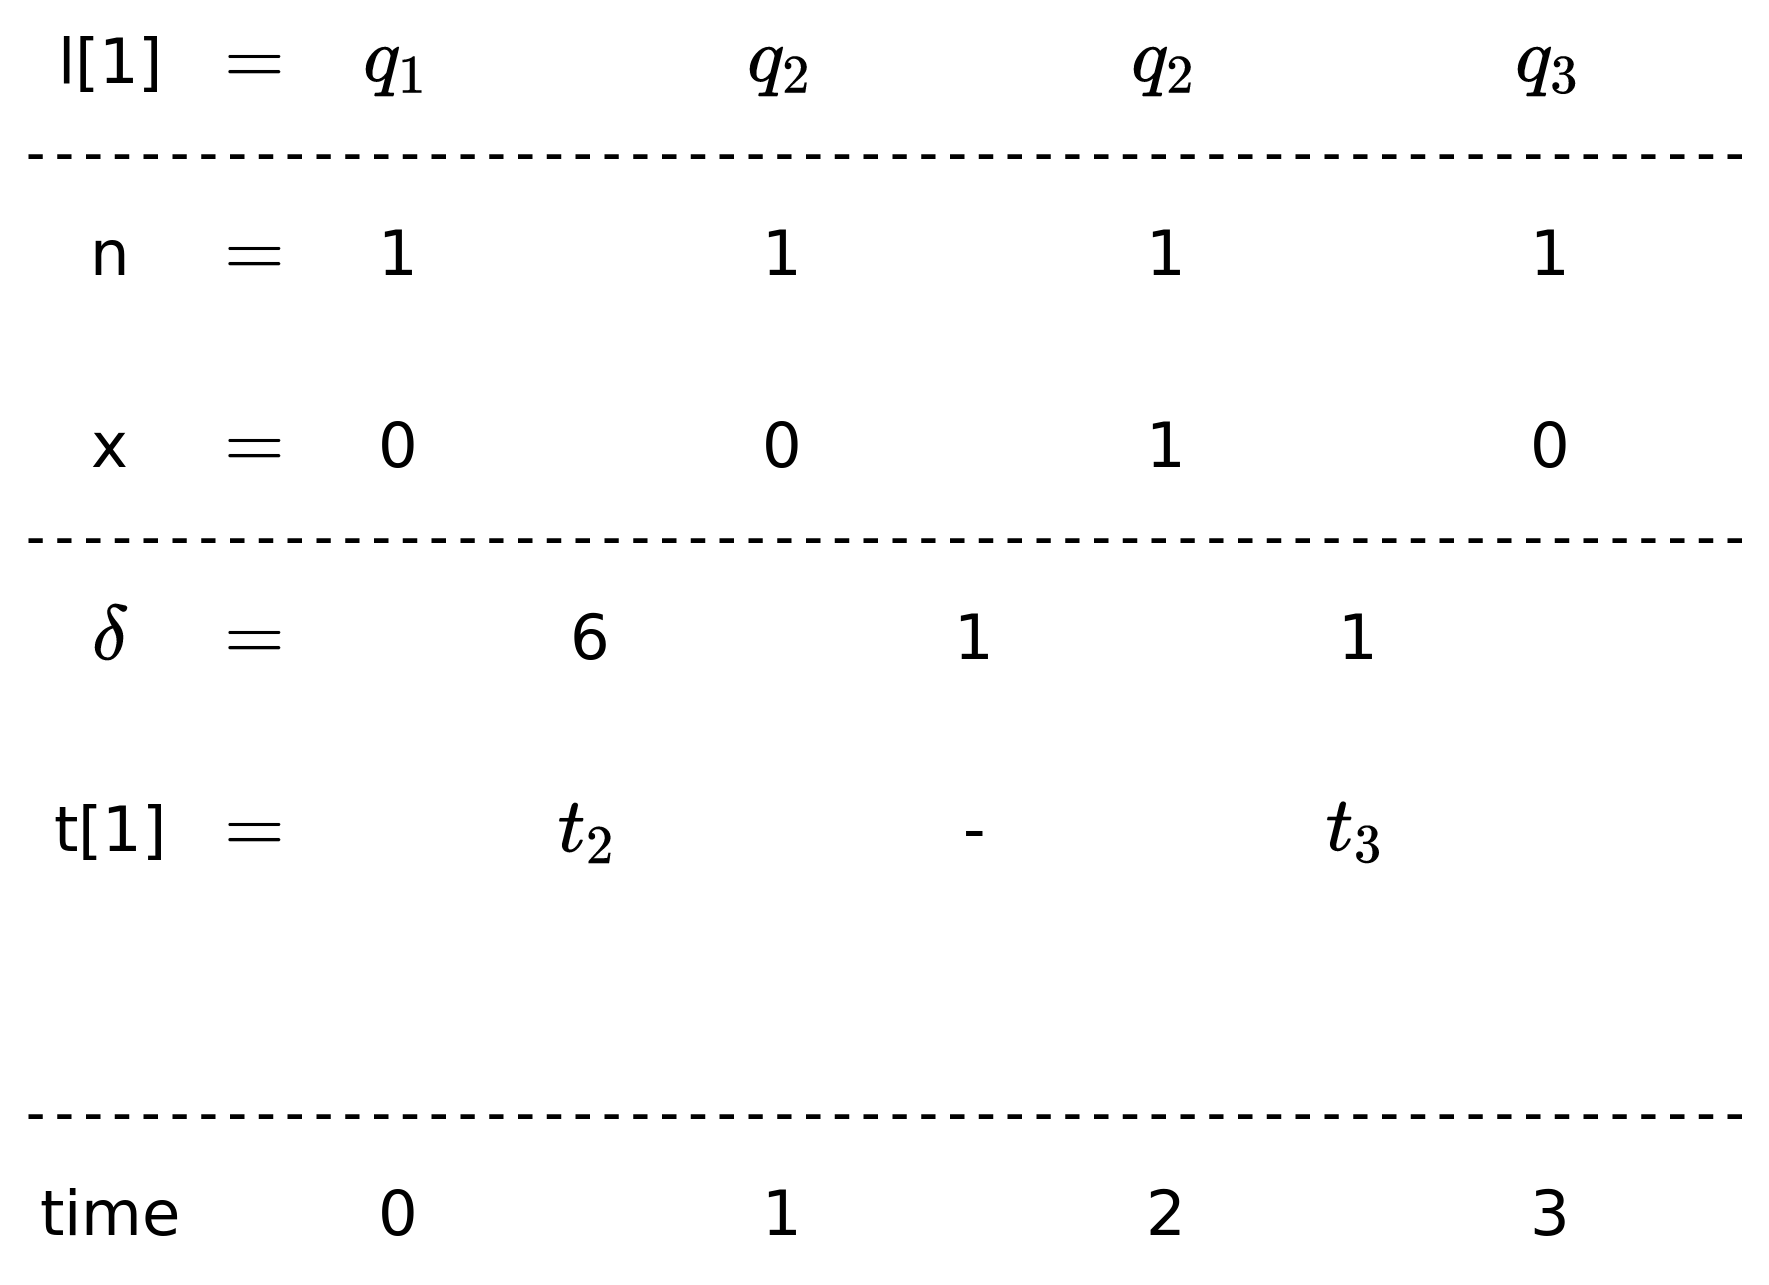
\includegraphics[width=0.6\textwidth]{trace-shift-min}
  \caption{An example trace through 4 positions.}
  \label{fig:trace-min}
\end{figure}

In Figure~\ref{fig:trace-min} we can see a trace of the Timed Automaton defined
in Figure~\ref{fig:example-big}, which has been given an index of 1. To prevent
the value of $t[i]$ being undefined at position $0$, the value of $t[i]$
corresponds to the transition taken in the following time position. However for
clarity in the traces shown here, the values of $t[1]$ have been shifted to the
right by one position, so that the active transition is placed over the position
in time where the transition actually occurs. At the top of the trace $l[1]$
tracks the currently active state of the timed automaton. In this simple trace
the automaton begins in state $q_{1}$, transitions to $q_{2}$, remains in
$q_{2}$ for another position, and then transitions to $q_{3}$. Below the active
state we show the active values of both the variable $n$ and the clock $x$ at
the given positions. The value $\delta$ shows the amount of time that passes
between the current state, and the immediately following state.

One surprising observation is that the value of the clock $x$ does not seem to
change between positions $0$ and $1$, despite $\delta$ indicating that $6$ units
of time has passed. Recall that transition $t_{2}$ resets the value of the clock
$x$ to zero, and that the trace capture the values of clocks and variables
\emph{after} any assignments have been applied.

\begin{figure}[h]
  \centering
  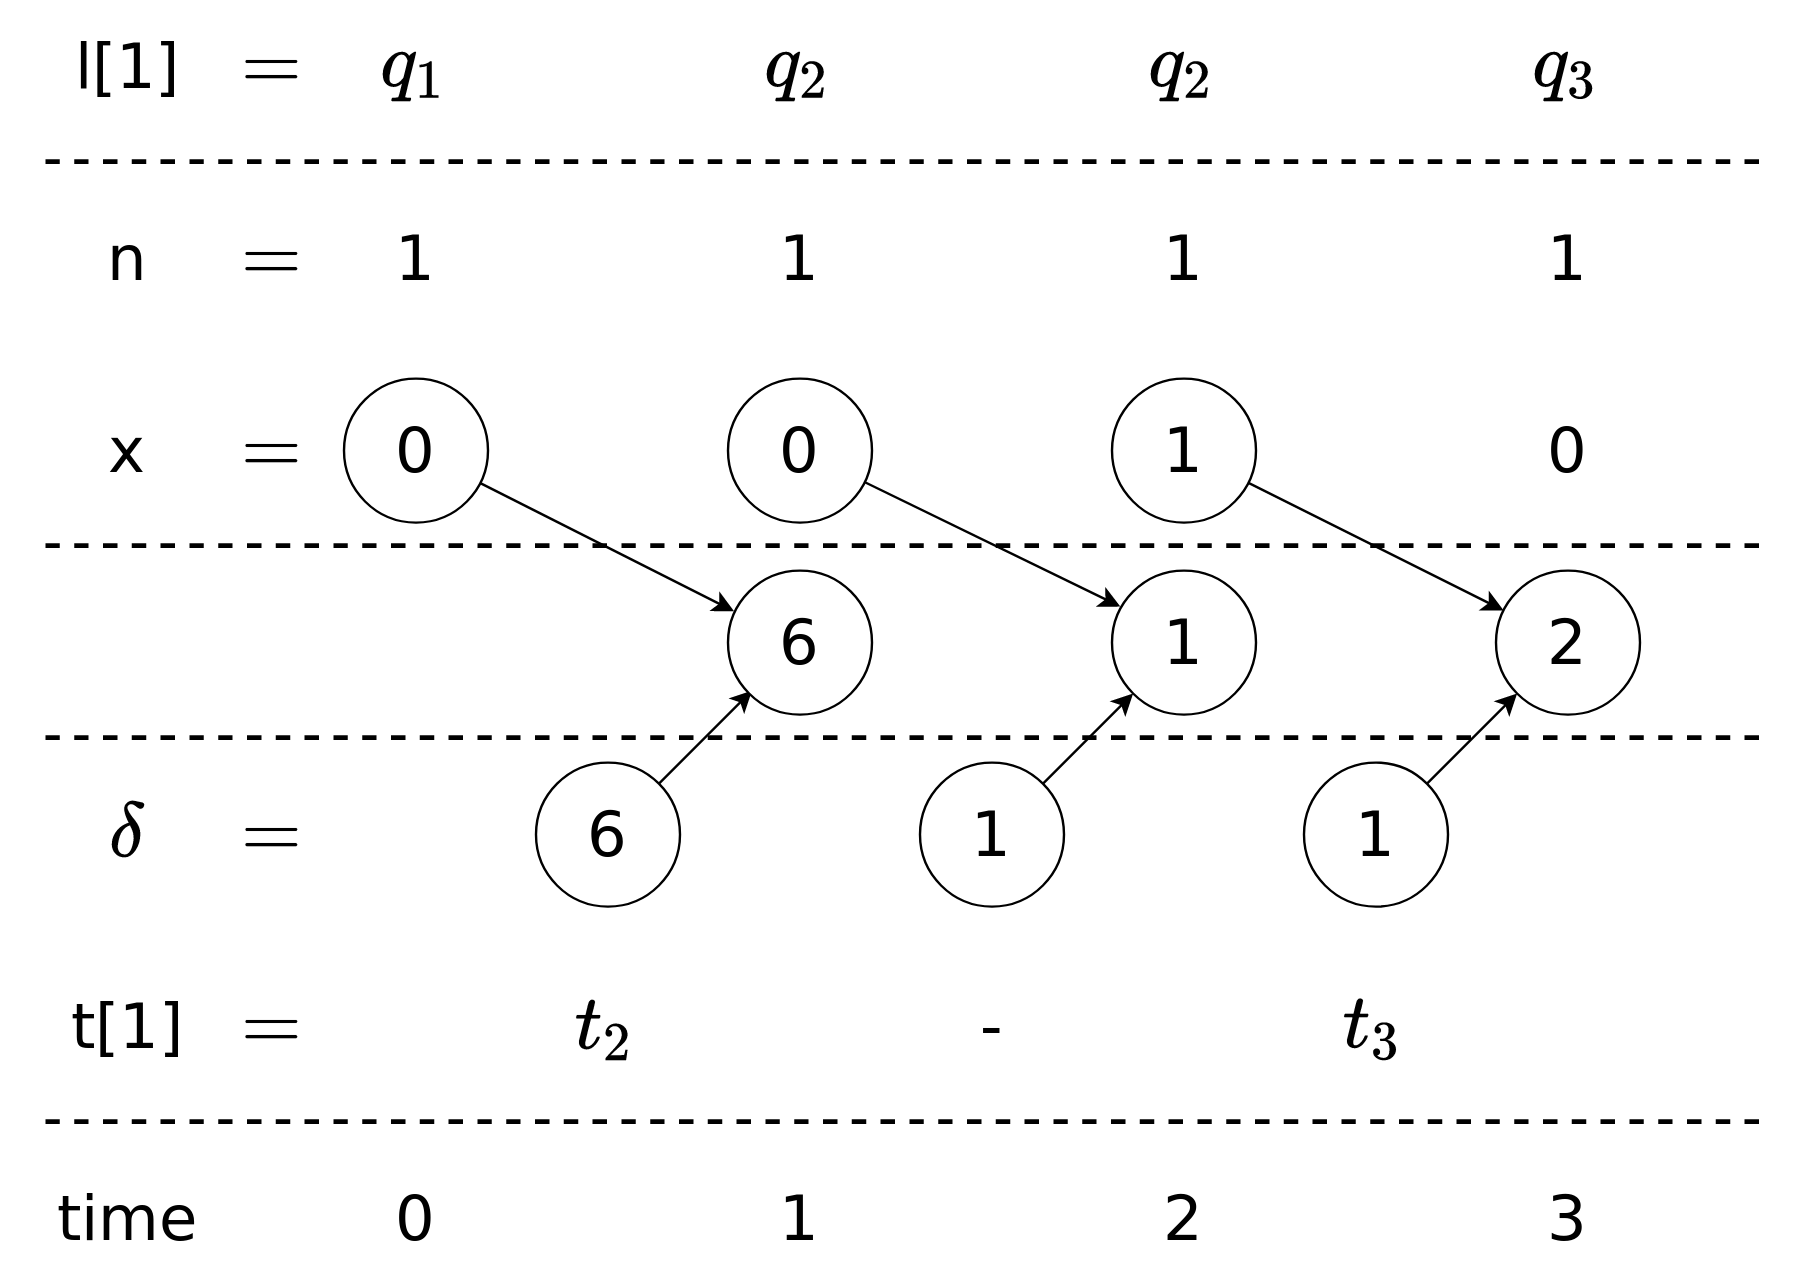
\includegraphics[width=0.6\textwidth]{trace-shift-delta}
  \caption{A trace highlighting the evaluation of a clock guard.}
  \label{fig:trace-delta}
\end{figure}

Figure~\ref{fig:trace-delta} shows how we can compute the value of clock $x$ at
the moment of the transition, before the reset is applied. By combining the
values of $x$ and $\delta$, we obtain the value of $x$ that is used to determine
if the clock guard of transition $t_{2}$ is satisfied. We see that $x$ has a
value of 6, which satisfies the guard $x>5$.

Notice in the above trace the value of clock $x$ during the transition from
state $q_{2}$ to state $q_{3}$. State $q_{2}$ has an invariant requiring that
the value of clock $x$ be strictly less than $2$, however at the moment of
transition $x(2) + \delta(2) = 2$. Is this trace therefore illegal? This raises
an interesting question: at the moment of transition, what is the active state?
Possible answers could include the source state, the destination, both, or
neither. Different models of Timed Automata implement this differently. Some,
like Uppaal~\cite{larsen97} implement so called ``super-dense'' time semantics,
in which the TA may be in multiple states in the same time instance. In our
model, the TA is always in exactly one state at every instant in time. If at the
moment of transition the TA remains in the source state, the transition is said
to be ``right-closed'' or equivalently ``left-open'', because the interval of
time that the TA spends in \(t_{-}\) ends in a closed interval, while the
interval of time that the TA spends in \(t_{+}\) begins in an open interval.
Conversely if the TA is located in the destination state at the moment of
transition, we say that it is ``left-closed'', which also implies that it is
right-open. Returning to our example trace, if the timed automaton is not in
state $q_{2}$ in the instance of transition, then the strict inequality in the
state invariant can be satisfied with equality at the instance of transition,
since the automaton is not actually in that state at that final moment. To
formalize this notion we introduce the weak clock relation $\sim_{w}$, which is
defined as follows:
\begin{align*}
  x \sim_{w} c  \iff & (x \sim c\ \lor\ x = c) \ \ \sim \in \{<,>,\leq,\geq\} \\
  x =_{w} c  \iff & false
\end{align*}
To make our trace more precise, we add for each TA $\mathcal{A}_{i}$ the term
$edge^{RC}[i]$, which is true at a given time position iff the currently active
edge is right-closed.

\begin{figure}[h]
  \centering
  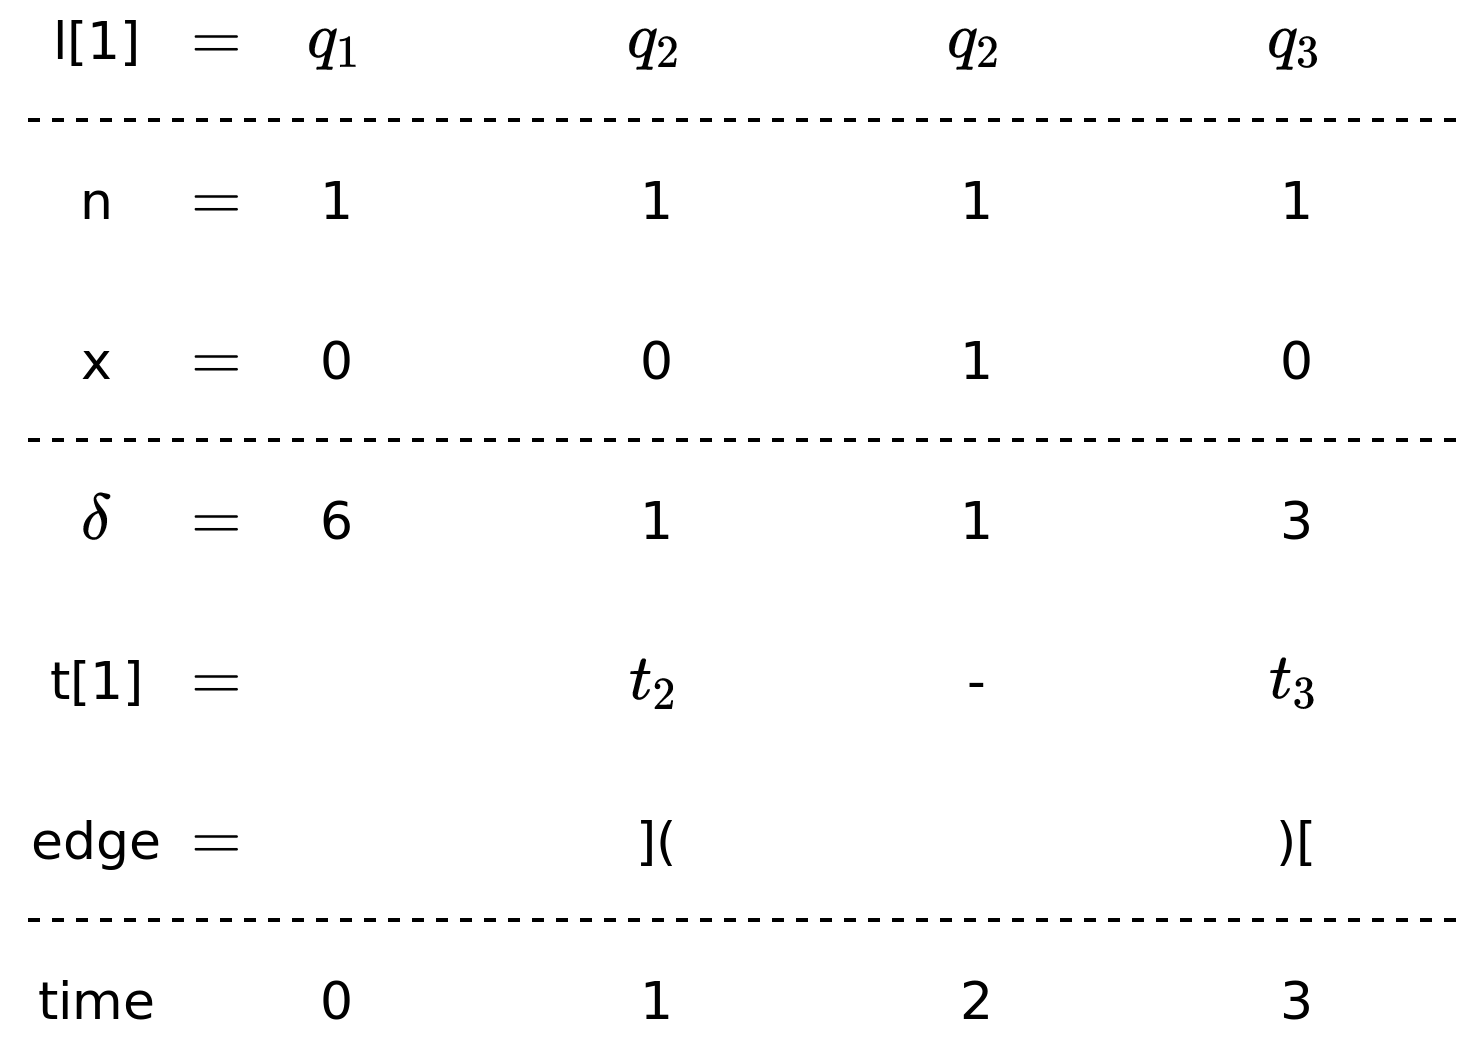
\includegraphics[width=0.6\textwidth]{trace-shift-full}
  \caption{An example trace with edge variable.}
  \label{fig:trace-full}
\end{figure}

Figure~\ref{fig:trace-full} shows the same example trace as before, but with the
addition of the edge variable. Like the transitions, it is shifted to the right
by one position for ease of viewing. Notice that when transition $t_{3}$ is
taken, the edge is left-closed, as is required by the invariant. The value of
the edge variable is not shown during the null transition, however during a null
transition either value is equivalent. We now revise the notion of a trace to
include this term.
\begin{defn} A trace $\eta$ is an infinite sequence
  \[\eta = (l_{0},v_{0},v_{var,0}),\delta_{0},t_{0},edge_{0}(l_{1},v_{1},v_{var,1}),\delta_{1},t_{1},edge_{1} \ldots\]
\end{defn}

When using Timed Automata to model real-time systems, a common desire is to
verify that every valid trace of the system obeys a given constraint, or
property. Problems of feasibility quickly arise however, due to the infinite
length of these traces. Bounded Model Checking is a process in which timed
automata traces of infinite length can be efficiently verified against a
property. Since TA traces are infinite in length, we restrict ourselves to
traces of the form
\(s_0 s_1\ldots s_{l-1}{(s_l s_{l+1}\ldots s_{k-1}s_k)}^\omega\), where every
$s = (l,v,v_{var},\delta,t)$. These ``lasso-shaped'' traces consist of an
initial sequence of states up until \(s_{l-1}\), followed by a loop that can be
repeated an infinite amount of times to form the full trace. Since the beginning
of the loop is allowed to occur anywhere within the sequence, the only variable
is the number of distinct states \(k\). Bounded Model Checking refers to
checking if a given property is satisfied over lasso-shaped traces of up to
length \(k\). The TA system along with the desired property are converted into a
format suitable for parsing by a SAT or SMT solver, which is then tasked with
finding a counterexample to the property. If a counterexample is found, then
there exists at least one trace that does not satisfy the provided property.
Otherwise, the property is said to have been verified over the TA network up to
the bound \(k\), as the solver has shown that no lasso-shaped traces of length
\(k\) exist that contradict the property. Although restricting ourselves to only
lasso-shaped traces may seem to be a severe limitation, it has been shown that
for a given TA network $\mathcal{A}$, there exists a limit $K$ such that if a
counterexample for a given property exists, there exists a lasso-shaped
counterexample of length no more than $K$~\cite{biere99}.

\section{Constraint LTL Over Clocks}\label{cltloc}

Constraint LTL is an extension of linear temporal logic allowing formulas over a
given constraint system~\cite{demri07}. \cltloc\ is a constraint LTL where the
constraint system consists of clocks defined over the positive real numbers.
This allows for the construction of formulas defined over atomic propositions
and clocks. A clock is a variable over \(\mathbb{R}_{\geq 0}\) whose value
changes between LTL positions to model the passage of time. Like clocks in timed
automata, clocks can be reset back to zero. In addition \cltloc\ has been
extended to support expressions over arithmetical variables~\cite{marconi16}.

A formula in \cltloc\ consists of atomic propositions, clock formulas, and
formulas over integer variables, which are combined using the standard LTL
operators of \(\mathcal{X}\) (next) and \(\mathcal{U}\) (until), as well as the
derived operators \(\mathcal{G}\) (globally), \(\mathcal{F}\) (future), and
\(\mathcal{R}\) (release). A clock formula compares the value of the clock to a
given natural number, for instance \(x > 7\). A variable formula, on the other
hand, can compare not only individual variables but also arithmetic combinations
of variables. An example would be the expression \(b + c = 7\); \(b,c \in Int\).

Let \(X\) be a finite set of clocks and \(Int\) be a finite set of integer
variables. \cltloc\ formulas are defined as follows:
\[\phi := p \BitOr x \sim c \BitOr \exp_{1} \sim \exp_{2} \BitOr \mathcal{X}(n) \sim \exp \BitOr \phi \land \phi \BitOr \neg \phi \BitOr \mathcal{X}\phi \BitOr \phi \mathcal{U} \phi \]
Where \(a \in AP\), \(x \in X\), \(c \in \mathbb{N}\), \(n \in Int\),
$\sim \in \{<,=\} $ and \(exp\) are arithmetic formulas over integer variables
and integers (defined in Section~\ref{timed-automata}).

As mentioned before, clocks are special dense variables over
\(\mathbb{R}_{\geq 0}\) that `progress' between different LTL positions. To be
more specific, each clock must either increment between two adjacent time
positions, or it must be reset. To maintain a consistent view of time, we
introduce \(\delta: \mathbb{N} \rightarrow \mathbb{R}_{>0}\), which measures the
amount of time that elapses between two adjacent time positions. For a given
clock `valuation'
\(\sigma: \mathbb{N} \times X \rightarrow \mathbb{R}_{\geq 0}\), each clock
\(x \in X\) must either obey the equivalence
\(\sigma(l,x) + \delta(l) = \sigma(l+1,x)\), or is reset, i.e.\
\(\sigma(l+1,x) = 0\). This ensures that all clocks progress at the same rate,
and we can use \(\delta(t)\) to calculate the amount of time elapsed between any
two positions.

We also define variables via the assignment function
$\iota : \mathbb{N} \times Int \rightarrow \mathbb{Z}$ that assigns a value to
each variable $n \in Int$ at every time position in $\mathbb{N}$. The
arithmetical expressions $\exp$ can now be evaluated at a time position $l$ by
replacing every occurrence of an integer variable $n$ with $\iota(l,n)$.

A \cltloc\ interpretation is the triple $(\pi, \sigma, \iota)$, where
$\phi: \mathbb{N} \rightarrow \wp(AP)$ maps time positions to the set of atomic
propositions that evaluate to true, and $\sigma$ and $\iota$ are the clock and
variable valuations. A \cltloc\ formula $\phi$ evaluated at time position $l$ is
defined as follows:
\begin{align*}
  &(\pi,\sigma,\iota),l \vDash x \sim c && \Leftrightarrow && \sigma(l,x) \sim c \\
  &(\pi,\sigma,\iota),l \vDash \exp_{1} \sim \exp_{2} && \Leftrightarrow && \exp_{1}(\iota,l) \sim \exp_{2}(\iota,l) \\
  &(\pi,\sigma,\iota),l \vDash \mathcal{X}(n) \sim \exp && \Leftrightarrow && \iota(l{+}1,n) \sim \exp(\iota,l) \\
  &(\pi,\sigma,\iota),l \vDash p && \Leftrightarrow && p \in \pi(l) \\
  &(\pi,\sigma,\iota),l \vDash \neg \phi && \Leftrightarrow && \neg ((\pi,\sigma,\iota),l \vDash \phi) \\
  &(\pi,\sigma,\iota),l \vDash \phi_{1} \land \phi_{2} && \Leftrightarrow &&((\pi,\sigma,\iota),l \vDash \phi_{1}) \land ((\pi,\sigma,\iota),l \vDash \phi_{2}) \\
  &(\pi,\sigma,\iota),l \vDash \mathcal{X}(\phi) && \Leftrightarrow && (\pi,\sigma,\iota),l{+}1 \vDash \phi \\
  &(\pi,\sigma,\iota),l \vDash \phi_{1} \mathcal{U} \phi_{2} && \Leftrightarrow &&((\pi,\sigma,\iota),l \vDash \phi_{2}) \lor \\
  &&&&& \bigg(((\pi,\sigma,\iota),l \vDash \phi_{1}) \land ((\pi,\sigma,\iota),l{+}1 \vDash \phi_{1} \mathcal{U} \phi_{2}) \bigg) \\
\end{align*}
A \cltloc\ formula $\phi$ is said to be \emph{satisfiable} if an interpretation
$(\pi,\sigma,\iota)$ exists such that $(\pi,\sigma,\iota),0 \vDash \phi$. This
is often shortened to simply $(\pi,\sigma,\iota) \vDash \phi$.


\section{MITL}\label{mitl}

Metric Interval Temporal Logic is a restriction of Metric Temporal Logic (MTL)
such that subscripts must be intervals~\cite{bouyer09}. An interval $I$ is a
convex region of $\mathbb{R}_{\geq 0}$. The bounds of this region must be in the
set $\{\mathbb{N} \cup \infty\}$. We will represent an interval as
$\langle a,b \rangle$ or $\langle a,\infty )$, where $a,b \in \mathbb{N}$,
$\langle\ \in \{\ (,[\ \}$ and $\rangle \in \{\ ),]\ \}$.

The following grammar describes the set of MITL formulas:
\[\phi := \alpha\ |\ \phi \lor \phi\ |\ \neg \phi\ |\ \phi\ \mathcal{U}_{I} \phi\]
Where $\alpha$ represents the set of atomic propositions. The set of
propositions currently supported by TACK consists of the set $AP$ (atomic
propositions of the network of TA) and propositions of the form $n = c$, where
$n$ is an integer variable and $c$ is a constant value.

The semantics of MITL are defined as follows. An MITL signal is a function
$M : \mathbb{R}_{\geq 0} \rightarrow \mathcal{P}(AP) \times \mathbb{Z}^{Int}$.
At a given time $t$, $M(t) = P, v_{var}$ gives us the set of $AP$ that evaluate
to true $P$, as well as a valuation for the integer variables $v_{var}$. For a
given signal $M$, $M,t \vDash \phi$ is defined as follows:
\begin{align*}
  &M,t \vDash \alpha && \Leftrightarrow && M(t) = (\psi,v_{var}) \land \alpha \in \psi \\
  &M,t \vDash n = c && \Leftrightarrow && M(t) = (\psi,v_{var}) \land v_{var}(v) = c \\
  &M,t \vDash \phi_{1} \land \phi_{2} && \Leftrightarrow && (M,t \vDash \phi_{1}) \land (M,t \vDash \phi_{2}) \\
  &M,t \vDash \neg \phi && \Leftrightarrow && \neg (M,t \vDash \phi) \\
  &M,t \vDash \phi_{1} \mathcal{U}_{I} \phi_{2} && \Leftrightarrow && \exists t' > t, t' - t \in I, (M,t \vDash \phi_{2}) \land \forall t'' \in (t,t'), (M,t'' \vDash \phi_{1}) \\
\end{align*}

An MITL formula $\phi$ is said to be \emph{satisfiable} if an interpretation
$M$ exists such that $M,0 \vDash \phi$. We then say that $M$ models $\phi$.


\section{TACK \cltloc\ Translation}\label{prelim-tack}

The TACK~\cite{tack20} tool developed by Menghi et al.\ converts Bounded
Satisfiability Checking problems into the CLTLoc language. TACK uses Metric
Interval Temporal Logic to specify the property to be checked for satisfiability,
which allows for more compact and powerful specifications of the desired
properties to be checked. Once the Timed Automata network and the MITL property
have been converted into CLTLoc, TACK then uses the tool Zot to convert this
intermediate representation of the problem into the SMT-LIB2 language, which is
supported by many modern SMT solvers. Zot was designed with a modular
architecture to allow for several different strategies and algorithms that can
be used to convert its input. Currently the most successful Zot plugin for
CLTLoc Bounded Model Checking is \aez. We will provide an overview of both
the TACK encoding of Timed Automata in CLTLoc and the ae2sbvzot translation of
CLTLoc into BitVector form.


Each time position in an infinite trace of a network of timed automata is
represented as a position in the mono-infinite temporal space of \cltloc. At
every time position $l[i]$ and $t[i]$ return the active state and active
transition at the current time position. Each function is syntactic sugar for a
set of atomic propositions, one for each possible value of the function, that
are constrained so that only one may evaluate to true in each time position.
Each $edge_{i}^{RC},\ i \in [1,N]$ is encoded as an atomic proposition. TA
clocks and variables can be represented directly as \cltloc\ clocks and
variables.


\begin{table}
  \centering
  % \setlength{\tabcolsep}{4pt}
  \aboverulesep=0ex
  \belowrulesep=0ex
  \renewcommand{\arraystretch}{1.2}
  \caption{TACK Encoding of an Automaton in CLTLoc}
  \label{tack-encoding}
  \begin{tabular}{c|c|c}
    \toprule
    \(\varphi_{1} := \underset{i \in [1,N]}{\bigwedge} (l[i] = 0)\) &
                                                                 \(\varphi_{2} := \underset{n \in Int}{\bigwedge} n = v_{var}^0 (n) \) &
                                                                                                                                     \(\varphi_{3} := \underset{i \in [1,N]}{\bigwedge} Inv(l[i])\) \\
    \midrule
    \(\varphi_{4} {:=} \underset{x \in X}{\bigwedge} (x_{0} {=} 0 \land x_{1} {>} 0 \land x_{v} {=} 0)\) &  \multicolumn{2}{c}{\( \varphi_{5}(j) {:=} \underset{x \in X}{\bigwedge} (x_{j} {=} 0) {\rightarrow} \mathcal{X}\left( (x_{(j{+}1){\mod 2}} = 0) \mathcal{R}\big( (x_{v}{=}j){\land}(x_{j}{>}0) \big) \right) \)} \\
    \midrule
    \multicolumn{3}{c}{\(\varphi_{6} := \underset{q \in \mathcal{Q}_{i}}{\underset{i \in [1,N]}{\bigwedge}} \bigg( \Big( l[i] = q \land t[i] = \sharp \Big) \rightarrow \mathcal{X} \Big( Inv(q) \land r_{1}(Inv(q)) \Big) \bigg) \)} \\
    \midrule
    \multicolumn{3}{c}{\( \varphi_{7} := \underset{t \in T_{i}}{\underset{i \in [1,N]}{\bigwedge}} t[i] = t \rightarrow \Big( l[i] = t_{-} \land \mathcal{X}(l[i] = t_{+}) \land \varphi_{\gamma_{c}} \land \varphi_{\gamma_{v}} \land \varphi_{\alpha_{c}} \land \varphi_{\alpha_{v}}  \land \varphi_{edge}(t_{-}, t_{+}, i) \Big) \)} \\
    \multicolumn{3}{c}{\( \varphi_{edge}(a,b,i) := \varphi_{\alpha RC}(a,b,i) \lor \varphi_{\alpha LC}(a,b,i) \)}
    \\
    \multicolumn{3}{c}{\( \varphi_{\alpha RC}(a,b,i) := Inv(a) \land r_{2}(Inv_{w}(b)) \land edge^{RC}[i] \)} \\
    \multicolumn{3}{c}{\( \varphi_{\alpha LC}(a,b,i) := Inv_{w}(a) \land r_{2}(Inv(b)) \land \neg edge^{RC}[i] \)} \\
    \midrule
    \multicolumn{3}{c}{\( \varphi_{8} := \underset{i \in [1,N]; q,q' \in \mathcal{Q}_{i} | q \neq q'}{\bigwedge} \bigg( \Big( (l[i] = q) \land \mathcal{X}(l[i] = q') \Big) \rightarrow \underset{t \in T_{i} | t_{-} = q, t_{+} = q'}{\bigvee} (t[i] = t) \bigg) \)} \\
    \midrule
    \multicolumn{3}{c}{\( \varphi_{9} := \underset{x \in X}{\bigwedge} \bigg( \mathcal{X}(x_{0} = 0 \lor x_{1} = 0) \rightarrow \underset{t \in T_{i} | x \in t_{a_{c}}}{\underset{i \in [1,N]} {\bigvee}} t[i] = t \bigg) \)} \\
    \midrule
    \multicolumn{3}{c}{\( \varphi_{10} := \underset{n \in Int}{\bigwedge} \bigg( (\neg(n = \mathcal{X}(n))) \rightarrow \underset{t \in T_{i} | n \in t_{a_{v}}}{\underset{i \in [1,N]}{\bigvee}} t[i] = t \bigg) \)}
  \end{tabular}
\end{table}

Table~\ref{tack-encoding} contains the formulas used to encode the Timed
Automata into CLTLoc. To accomplish this encoding, several auxiliary formulas
are used. \(l[i], i \in [1,N]\) represents the \emph{location} of the TA \(i\)
at the current time position. Likewise, \(t[i], i \in [1,N]\) represents the
currently active transition for TA \(i\) at the current time position. Because
not every TA will transition at each time position, we introduce a \emph{null
  transition} symbol \(\sharp\). Therefore the function \(t[i]\) may return
either a transition or the symbol \(\sharp\). If transition \(t\) is active in a
given position \(i\), then the TA is in state \(t_{-}\) at position \(i\) and
state \(t_{+}\) at position \(i+1\).

The first formula constrains each TA to be in the initial state at time 0. For
each Timed Automaton, the states are represented as natural numbers, with the
initial state as \(0\). The second formula initializes each variable
\(n \in Int\) to its initial value, and the third ensures that the invariants of
each initial state hold in the initial position.

% TODO: clocks?
Formulas 4 and 5 are the clock constraints, and describe how the active value of
the clock evolves throughout the trace. To both test the value of a clock and
simultaneously reset the value during a transition, TACK has used two clock
variables to encode a single clock value. There is currently a work in progress
to extent \cltloc\ to support simultaneous test and reset, however at the time
of writing this is not published. For a clock $x$, $x_{v}$ holds the index of
the active clock value, and references to the clock value elsewhere are
syntactic sugar for evaluating this variable and then choosing the appropriate
clock value. The active value is never zero, and a clock reset at position $i$
is not reflected in the formula until position $i{+}1$.

Formula $\varphi_{6}$ defines the semantics for the null transition. If a Timed
Automaton performs a null transition then at the moment of transition, the state
invariant must hold both before and after clock resets are applied. The function
$r_{1}$ replaces the value of any reset clock with $0$, thus capturing the
post-reset value of any clock used in the invariant.

Formula $\varphi_{7}$ encodes the discrete transitions. Each must respect the guards
and assignments of the transitions, the TA must currently be in the source state
of the transition, and must be in the destination state in the following
position. $\varphi_{edge}$ encodes the two possible edge states, right and
left-closed, and ensures that the invariants are satisfied, either weakly or
strongly depending on the edge type. Function $r_{2}$ again ensures that in the
event of a clock reset, the the invariants of the destination state are
evaluated against the correct clock values.

The final three formulas capture the sufficient conditions for a discrete
transition. The active state of a TA my not change, nor may a clock be reset,
nor may a variable value change without a transition explicitly causing the
change.

\begin{table}[ht]
  \centering
  \renewcommand{\arraystretch}{1.5}
  \begin{tabular}{l c c}
    \toprule
    \textbf{Type} && \textbf{Synchronization Encoding} \\
    \midrule
    \multirow{2}{5em}{One-to-one}
                  & $v_{1} :=$ &
                                 $\underset{t \in T_{i}| t_{\epsilon} = \alpha!}{\underset{i \in [1,N]}{\land}} \Bigg( t[i] = t \rightarrow \underset{j \neq i}{\underset{j \in [1,N],}{\lor}} \Bigg( \genfrac{}{}{0pt}{0}{\genfrac{}{}{0pt}{0}{\varphi_{sync{\mhyphen}on}(j,\alpha?) \land \neg \varphi_{sync{\mhyphen}on{\mhyphen}but}(\{i,j\},\alpha?)}{\land}}{\varphi_{same{\mhyphen}edge}(i,j)} \Bigg) \Bigg)$
    \\
                  & $v_{2} :=$ &
                                 $\underset{t \in T_{i}| t_{\epsilon} = \alpha?}{\underset{i \in [1,N]}{\land}} \Bigg( t[i] = t \rightarrow \underset{j \neq i}{ \underset{j \in [1,N],}{\lor}}( \varphi_{sync{\mhyphen}on}(j,\alpha!) \land \neg \varphi_{sync{\mhyphen}on{\mhyphen}but}(\{i,j\}, \alpha!) ) \Bigg)$
    \\
    \midrule
    \multirow{2}{5em}{Broadcast}
                  & $v_{1} :=$ & $\genfrac{}{}{0pt}{0}{\genfrac{}{}{0pt}{0}{\underset{t \in T_{i}|t_{\epsilon} = \alpha \#}{\underset{i \in [1,N]}{\bigwedge}} (t[i] = t \rightarrow (\neg \varphi_{sync{\mhyphen}on{\mhyphen}but}(\{i\},\alpha \#)))}{\land}}{\underset{t \in T_{i}|t_{\epsilon}=\alpha \#}{\underset{i \in [1,N]}{\bigwedge}} \bigg( t[i]=t \rightarrow \bigg( \underset{j \neq i}{\underset{h \in [1,N]}{\bigwedge}} \bigg( \genfrac{}{}{0pt}{0}{\genfrac{}{}{0pt}{0}{\varphi_{sync{\mhyphen}on}(j,\alpha @) \land \varphi_{same{\mhyphen}edge}(i,j)}{\lor}}{\big( \underset{t_{\epsilon}' = \alpha @}{\underset{t' \in T_{i'},}{\bigwedge}} (\mathcal{X}(\neg \phi_{t_{\gamma_{c}}'}) \lor \neg \phi_{t_{\gamma_{v}}'} \lor l[j] \neq {t'}_{-}) \big)} \bigg) \bigg) \bigg)}$
    \\
                  & $v_{2} :=$ & $\underset{t \in T_{i}|t_{\epsilon} = \alpha @}{\underset{i \in [1,N]}{\land}} (t[i] = t \rightarrow \varphi_{sync{\mhyphen}on{\mhyphen}but}(\{i\},\alpha\#))$\\
    \midrule
                  $\varphi_{sync{\mhyphen}on}$&$(j,\alpha):=$ &$\underset{t \in T_{i} | t_{\epsilon} = \alpha}{\bigvee} (t[i] = t)$\\
                  $\varphi_{sync{\mhyphen}on{\mhyphen}but}$&$(S,\alpha):=$ & $\underset{g \in \{i|i \in [1,N]\}\backslash S}{\bigvee} \varphi_{sync{\mhyphen}on}(h,\alpha)$\\
                  $\varphi_{same{\mhyphen}edge}$&$(i,j):=$ & $\mathcal{X}(edge^{RC}[i] \leftrightarrow edge^{RC}[j])$\\
    \bottomrule
  \end{tabular}
  \caption{Encoding of Different Synchronization Types}
  \label{table:cltloc-sync}
\end{table}

Table~\ref{table:cltloc-sync} contains the encodings for the two supported
synchronization types. These synchronization semantics are defined in
Table~\ref{table:sync-def}. The formula \emph{sync-on} is true if the automaton
$i$ performs a transition with the event $\alpha$. \emph{Sync-on-but} is true if
an automaton not included in the set $S$ performs a sync on $\alpha$.
\emph{Same-edge} is true if the two automatons have the same edge type.


\emph{Liveness Constraints} When we introduced the concept of traces, we gave
examples in which at least one Timed Automata performed a non-null (or discrete)
transition at every position in the trace. It seems natural to require at least
one discrete transition in each position, because otherwise the state of the
network would not change, and we could simply remove the unneccessary duplicate
position from the trace. Unfortunately the addition of MITL properties makes
this a bit more complex. Consider the MITL property
$\mathcal{G}_{[0,\infty)} \neg(\mathcal{G}_{[0,10]}\ \alpha)$, where $\alpha$ is
an atomic proposition which only evaluates to true in state $q$. This property
states that a TA is never in state $q$ for 10 or more time units before leaving.
Now let us consider a hypothetical counterexample. In trace $\eta$, the TA
transitions into state $q$ at position $i$, and then transitions to another
state in position $i{+}i$, with $\delta(i)=20$. This clearly violates the
property, as the TA remained in state $q$ for 20 seconds. However in order to
detect this violation, the MITL encoding requires there to be a specific
position in which the property is violated. Unfortunately position $i{+}1$ does
not suffice, as the TA is no longer in the critical state $q$. This
counterexample can only be detected if the solver has the ability to add another
time position in-between $i$ and $i{+}1$, where at least 10 units of time has
passed \textbf{and} the TA is still located in state $q$. Thus we must tolerate
positions in which every TA performs a null transition. That being said, we
often do not wish to accept traces in which discrete transitions \textbf{never}
occur. These requirements are termed \emph{liveness constraints}.


\begin{table}[h]
  \centering
  \begin{tabular}{p{0.2\textwidth} p{0.1\textwidth} c}
    \toprule
    \textbf{Type} && \textbf{Liveness Semantics} \\
    \midrule
    Strong transition liveness &&
                                 $\underset{i \in [1,N]}{\land} \mathcal{G}(\mathcal{F}(t[i] \neq \sharp))$
    \\
    \midrule
    Weak transition liveness && $\mathcal{G}(\mathcal{F}(\underset{i \in [1,N]}{\lor} t[i] \neq \sharp))$ \\
    \midrule
    Unrestricted && $\top$ \\
    \bottomrule
  \end{tabular}
  \caption{Possible Liveness Constraints}
  \label{table:liveness-def}
\end{table}

In addition to the TA and synchronization constraints, TACK includes support for
optional liveness constraints. The first is termed Strong Transition Liveness,
which is shown in Table~\ref{table:liveness-def}. This guarantees that every
time position, eventually in the future all timed automaton in the network will
take a discrete transition. Although a weaker version termed Weak Transition
Liveness is defined in the TACK paper, it is not implemented in the TACK tool.
It requires that at every position \emph{at least one} timed automaton will
eventually perform a discrete transition. Finally the Unrestricted Liveness
option places no restrictions on TA liveness.
%todo liveness background?

\begin{table}[h]
  \centering
  \begin{tabular}{l c c}
    \toprule
    \textbf{Type} &\quad\quad\quad\quad & \textbf{Edge Semantics} \\
    \midrule
    Right-closed & & $\underset{i \in [1,N]}{\land} \mathcal{G} (edge^{RC}[i])$ \\
    \midrule
    Open & & $\top$ \\
    \bottomrule
  \end{tabular}
  \caption{Possible Edge Constraints}
  \label{table:edge-def}
\end{table}

\emph{Edge Constraints} In addition to liveness, TACK also allows for
customization of its edge constraints. As we have seen in
Section~\ref{bounded-sat}, the edge variables are necessary for defining which
state an automaton is located in during the instant of transition. However the
freedom to choose between two possible edge types is often not needed, and adds
additional overhead to the solver. To speed up problems that do not have
invariant edge cases, TACK provides the option to set all edge variables to
right-closed in every time position. As seen in Table~\ref{table:edge-def}, this
is contrasted with the `open' edge semantics, which do not place any additional
restrictions on the edge variables.


\section{Bit-Vector Logic}\label{bvlogic}
A BitVector is an array of binary values, or bits. BitVectors are interpreted
using two's complement arithmetic to produce integer values, and their length
can be any positive integer (\(\mathbb{Z}^+\)). We use the notation
\(\overleftarrow{x}_{[n]}\) to represent a BitVector \(x\) of length \(n\), but
this can be simplified to \(\overleftarrow{x}\) if the length is clear. Bits are
numbered from right to left, with the rightmost, least significant bit labeled
as 0, and the leftmost, most significant bit labeled as \(n-1\). As an example,
the constant vector \(-4\) of length 5 would be written as
\(\overleftarrow{-4}_{[5]}\), which would expand to \(11100\). We can also
reference individual bits in the vector using the notation
\(\overleftarrow{x}_{[n]}^{[i]}\) to \(extract\) the \(i\)th bit from the
BitVector \(x\). It is also possible to extract a sub-vector with the notation
\(\overleftarrow{x}_{[n]}^{[j:i]}\), where \(n>j\geq i\geq 0\). This extracts a
vector of length \(j-i+1\) whose rightmost bit corresponds to the \(i\)th bit of
\(x\) and whose leftmost bit corresponds to the \(j\)th. Similarly,
\(concatenation\) operates on two BitVectors by combining their bit arrays.
\(\overleftarrow{x}_{[n]} :: \overleftarrow{y}_{[m]}\) returns a new BitVector
\(\overleftarrow{z}_{[n+m]}\) where \(\overleftarrow{z}^{[m-1:0]} =
\overleftarrow{y}\), and \(\overleftarrow{z}^{[m+n-1:m]} = \overleftarrow{x}\).

The usual arithmetic operations of addition (\(+\)) and subtraction (\(-\)) are
defined over two BitVectors of the same length. BitVectors also support the
bit-wise operators not (\(\BitNeg\)), disjuction (\(\BitOr\)), conjunction (\(\BitAnd\)),
equivalence (\(\iff\)), and implication (\(\Rightarrow\)). These binary operators return a
new BitVector where each bit \(i\) is the result of applying the logical
operator to the \(i\)th bit of each of the input vectors, following the usual
convention where \(1\) is true and \(0\) is false. For example, the expression
\(\big( \overleftarrow{1100} \Rightarrow \overleftarrow{1010} \big) \) would
evaluate to \(\overleftarrow{1101}\), since \(a \rightarrow b\) is equivalent to
\(a \lor \neg b\).

\section{AE2SBVZOT}\label{zot-encoding}

The final program to mention is \aez, which is a BitVector-based plugin for Zot.
It accepts CLTL formulas and converts them to BitVector logic, which it then
sends to Microsoft's Z3 to solve.

\begin{table}[hb]
  \centering
  \caption{An example \aez\ trace showing loop variables.}
  \begin{tabular}{l|c c c c c}
    BitVector & \textbf{4} & 3 & \textbf{2} & 1 & 0 \\
    \midrule
    \(\overleftarrow{foo}\)            & \textbf{1} & 0 & \textbf{1} & 1 & 0 \\
    \(\overleftarrow{\neg foo}\)       & \textbf{0} & 1 & \textbf{0} & 0 & 1 \\
    \(\overleftarrow{\mathcal{X}foo}\) & \textbf{0} & 1 & \textbf{0} & 1 & 1 \\

    \midrule
    \(\overleftarrow{lpos}\)           & 0 & 0 & 0 & 1 & 0 \\
    \(\overleftarrow{inloop}\)         & 1 & 1 & 1 & 0 & 0

  \end{tabular}
  \label{table:zotloop}
 \end{table}

To model the lasso shape of runs, \aez\ adds an additional position to the
BitVector that represents the `loopback' position, or the first position of the
next iteration of the loop. This position becomes the left-most, most
significant bit of the vector. To separate the lasso from the initial portion of
the trace, \aez\ defines two special BitVectors, \(\overleftarrow{lpos}\) and
\(\overleftarrow{inloop}\). In Table~\ref{table:zotloop} we can see an example formula,
\(foo\), along with the corresponding vectors \(\overleftarrow{lpos}\) and
\(\overleftarrow{inloop}\). We can see that \(\overleftarrow{lpos}\) has a value
of 2, meaning that bit 2 is the first position in the loop. Looking at the table
we can see that the columns for bits 2 and 4 are in bold, to represent that 4,
being the `loopback' position, is a copy of position 2, and therefore all
formulas are constrained to have identical values in these positions. Meanwhile
\(\overleftarrow{inloop}\) highlights that bits 0 and 1 are \textbf{not} in the
loop portion of the trace, while the rest of the positions are. The infinite
trace therefore would begin in position 0, move to position 1, and then repeat
the infinite sequence of positions \([232323\ldots]\).

\begin{table}[ht]
  \centering
  %\setstretch{0.7}
  \caption{\aez\ definition of a proposition \(\varphi\)}
  \begin{tabular}{c c}
    \(\phi\) & Encoding \\
    \midrule
    \(\neg \varphi\)                & \(\overleftarrow{(\neg \varphi)} =\BitNeg\overleftarrow{(\varphi)}\) \\
    \(\varphi_{1} \land \varphi_{2}\)& \(\overleftarrow{(\varphi_{1} \land \varphi_{2})} = \overleftarrow{(\varphi_{1})} \BitAnd \overleftarrow{(\varphi_{2})} \) \\
    \(\varphi_{1} \lor \varphi_{2}\)& \(\overleftarrow{(\varphi_{1} \lor \varphi_{2})} = \overleftarrow{(\varphi_{1})} \BitOr \overleftarrow{(\varphi_{2})} \) \\
    \midrule
   % \(\mathcal{Y}\varphi\)         & \(\overleftarrow{(\mathcal{Y}\varphi)} =\ \ll \overleftarrow{(\varphi)}\) \\
   % \(\varphi_{1}\mathcal{S}\varphi_{2}\) & \( \overleftarrow{(\varphi_{1}\mathcal{S}\varphi_{2})}^{[k{+}1:0]} = \biggl(\overleftarrow{(\varphi_{2})}^{[k{+}1:1]} \BitOr \bigl( \overleftarrow{(\varphi_{1})}^{[k{+}1:1]} \BitAnd \) \\
   %          & \(\overleftarrow{(\varphi_{1}\mathcal{S}\varphi_{2})}^{[k:0]}\bigr) \biggr) :: \overleftarrow{(\varphi_{2})}^{[0]} \) \\
    \(\mathcal{X} \varphi\)        & \(\overleftarrow{(\mathcal{X}\varphi)}^{[k:0]} = \overleftarrow{(\varphi)}^{[k{+}1:1]} \) \\
    \(\varphi_{1} \mathcal{U} \varphi_{2}\) & \(\overleftarrow{(\varphi_{1} \mathcal{U} \varphi_{2})}^{[k:0]} = \overleftarrow{(\varphi_{2})}^{[k:0]} \BitOr \bigl( \overleftarrow{(\varphi_{1})}^{[k:0]} \BitAnd \overleftarrow{(\varphi_{1} \mathcal{U} \varphi_{2})}^{[k{+}1:1]} \bigr) \) \\
             & \(\land \biggl( \Bigl( \big( \overleftarrow{(\varphi_{1})}^{[k{+}1]} \BitOr \overleftarrow{(\varphi_{2})}^{[k{+}1]} \BitOr \BitNeg\overleftarrow{(\varphi_{1} \mathcal{U} \varphi_{2})}^{[k{+}1]} \big) \BitAnd\) \\
             & \( \big( !\overleftarrow{(\varphi_{2})}^{[k{+}1]} \BitOr \overleftarrow{(\varphi_{1} \mathcal{U} \varphi_{2})}^{[k{+}1]}\big) \Bigr) = 1 \biggr) \land \) \\
    & \( \big( \overleftarrow{(\varphi_{1} \mathcal{U} \varphi_{2})}^{[k{+}1]} \Rightarrow \Uparrow \bigl( \overleftarrow{(\varphi_{2})} \BitAnd \overleftarrow{(inloop)} \bigr) = 1 \big) \)

  \end{tabular}
  \label{table:zot-constraints}
 \end{table}

Given a formula with a bound of \(k\), \aez\ constructs a BitVector for the
formula and for each sub-formula with a length of \(k{+}2\). It adds an extra
position both at the beginning (bit 0) to represent the initial configuration of
the system, as well as at the end (bit \(k{+}1\)) to represent the loopback
position as discussed. Each formula is then represented as a formula over its
component sub-formulas based on the rules in Table~\ref{table:zot-constraints}.
The first three formulas show the encoding of logical operators \(\neg, \land\),
and \(\lor\). The rest of the table shows the encoding of the temporal
operators. Extra care is taken in the definition of \(\mathcal{U}\) to ensure
that the properties of the lasso are taken into account.

%\begin{table}
%  \centering
%  \begin{tabular}{c}
%    $ \underset{t \in T}{\land} \overleftarrow{t}_{[k{+}2]}^{[loop]} = \overleftarrow{t}_{[k{+}2]}^{k{+}1}$
%    \\
%    $\underset{q \in Q}{\land} \overleftarrow{q}$
%  \end{tabular}
%\end{table}


Atomic propositions (including the active states, transitions, edges and
variable valuation) are encoded as BitVectors, and form the basic atoms from
which more complex expressions are built upon. For each state, transition, and
possible variable assignment (i.e.\ $n = 4$), there is a BitVector defined whose
value is $1$ if the corresponding state or transition is active, or if the
variable assignment is true. One limitation of this approach is that arithmetic
operations over variables cannot be represented. As a result, in this
implementation, variable guards may only test for equality, and different
variables cannot be added or subtracted in a variable assignment statement.

\begin{table}[hb]
\centering
\begin{tabular}{ll}
 Transition Bit & BitVector\\
\midrule
0 & \(\overleftarrow{tb_{i,0}}_{[k+2]}\)\\
1 & \(\overleftarrow{tb_{i,1}}_{[k+2]}\)\\
\rotatebox{90}{\ldots} & \rotatebox{90}{\ldots}\\
\((\lceil \log_2 T_i \rceil -1)\) & \(\overleftarrow{tb_{i,(\lceil \log_2 T_i \rceil -1)}}_{[k+2]}\)\\
\end{tabular}
\caption{Construction of the Transition BitVectors for \(\mathcal{A}_{i} \in \mathcal{A}\)}
\label{table:compact-bv}
\end{table}

To reduce the number of variables used, rather than store each transition
(respectively state, variable value) as a separate BitVector, \aez\ uses a more
compact bit-based representation. We will use transitions to illustrate this
encoding, which is identical for states and variables as well. Since only one
transition is active at a time, it is more compact to store the currently active
transition as a binary number over \(\lceil\log_2 |T|\rceil\) bits.
Therefore \aez\ creates \(\lceil\log_2 |T|\rceil\) BitVectors of
length \(k+2\) to represent the active transition of the TA over time.
Table~\ref{table:compact-bv} shows how these BitVectors are constructed to represent
the active transition of a single timed automaton. To reconstruct a BitVector
whose bits have the value of 1 iff a given transition $t$ is active, \aez\
combines the multiple transition bitvectors in a unique fashion to represent a
specific transition. As an example, consider a transition $t \in T_{i}$ that has
been encoded as the number $1$. Since the binary representation of $1$ is
$\overleftarrow{00\ldots}001$, to create the BitVector for transition $t$ \aez\
would construct the following expression:
\[\BitNeg\overleftarrow{tb_{i,\lceil \log_2 \mathcal{T}_i \rceil -1}} \BitAnd \ \BitNeg\overleftarrow{tb_{i,\lceil \log_2 \mathcal{T}_i \rceil -2}} \BitAnd \ldots \BitAnd \ \BitNeg\overleftarrow{tb_{i,1}} \BitAnd \overleftarrow{tb_{i,0}} \]
In this expression every BitVector is negated except for the last, which
corresponds to the number one. Each transition (resp.\ state, variable value) is
assigned a combination of the corresponding BitVectors in this fashion.


Clocks, being real-valued functions, cannot be easily represented in BitVector
logic. Instead \aez\ takes advantage of SMT-LIB2's support for multiple logics,
and encodes clocks directly as functions that accept an integer argument,
representing the time position, and return a real number. For a given clock
guard a BitVector is constructed to represent the truth value of the clock
expression. These can then be used to construct larger expressions using the
rules shown in Table~\ref{table:zot-constraints}.

Unlike the other terms, clocks cannot simply be constrained to hold the same
value in the loopback position. As shown by Kindermann~\cite{kindermann12} this
excludes certain valid lasso shaped traces. To avoid this \aez\ adopts the
region-based clock constraints suggested by Kindermann. Two clock valuations are
said to be in the same region if at both positions $loop$ and $k{+}1$:
\begin{itemize}
  \item Each clock $x$ is either greater than the maximum value compared against
    $x$ in a clock guard in both positions ($\lfloor x \rfloor > \max(x)$) or
    $\lfloor x(loop) \rfloor = \lfloor x(k{+}1) \rfloor$
  \item If $\lfloor x \rfloor \leq \max(x)$, the formula
    $x(l) - \lfloor x(l) \rfloor = 0$ must have the same value in both $loop$
    and $k{+}1$
  \item For every pair of clocks $x,x'$, if the floor of both clocks are less
    than their maximum values, then the formula
    $frac(x(l)) < frac(x'(l))$ must have the same value in positions $loop$ and
    $k{+}1$, where $frac$ is the fractional part of the clock's value.
\end{itemize}
These conditions are sufficient to ensure that the clock valuation in each
position belongs to the same region, a concept expanded on in Kindermann's
work~\cite{kindermann12}. This allows \aez\ to represent loops where the elapsed
time of each loop iteration is constrained to be less than the elapsed time of
the previous iteration. Although a lasso with a fixed amount of time per-loop
iteration does not exist, there exists infinite series of loop iterations, each
with a decreasing elapsed time, that nonetheless have a diverging sum, and thus
represent infinite traces.

Since the time per-loop iteration is no longer fixed, another constraint is
required to ensure that no ``Zeno-shaped'' traces are allowed. In Zeno traces,
the time elapsed in the infinite trace sums to a finite number. These cases are
considered pathological and to exclude them, it has been
proven~\cite{kindermann12} that it is sufficient to require that in the loop
section of the trace, that every clock is either
\begin{itemize}
  \item Reset at least once during the loop
  \item or has a value greater than $max(x)$ in the final loop position.
\end{itemize}
This concludes the \aez\ encoding of a \cltloc\ formula.

\chapter{Novel Encoding of Timed Automata Networks}\label{encoding}

The previous work in this field has relied on first translating the TA network
and property to be verified into the intermediate \cltloc\ representation, to be
later translated into BitVector logic and solved. Presented here is a novel
method, named ta2smt, in which the Timed Automata network is directly encoded
into BitVector logic. This direct translation allows us to make several
optimizations not possible in \cltloc. As before, the MITL property will
continue to be converted first into \cltloc\ before being transformed into
BitVector logic by \aez. We use a consistent naming convention for the atomic
propositions to ensure that the two BitVector encodings can be safely combined
to produce the final SMT output. This chapter is organized into three parts. In
the first, we describe the various terms that make up our TA network, and
discuss how they are encoded into BitVector logic. In the second, we present the
constraints, defined over the terms from the first section, that capture the TA
semantics. In the final section we argue for the correctness of our model, and
highlight improvements made over \aez.

\section{BitVectors}


Like \aez, our novel encoding (ta2smt) is based on encoding the terms of the
Timed Automata into BitVectors. Using BitVector logic, we have the ability to
group logically connected propositions into a Vector, granting significant
speedups on operations performed over every element of the vector. We wish to
use this property to group together logically connected constraints of the
encoding. One common source of constraint duplication is the transition
constraints. These constraints enforce the semantics of Timed Automaton
transitions, requiring that, for example all guards and assignment statements
have been fulfilled. These constraints must be upheld at every transition in the
trace, which can be dozens of discrete transitions long. This motivates us to
use the BitVectors to represent a piece of information changing over time, i.e.\
representing its value at different time positions in the trace.

%When encoding the constraints of the system, it is convenient to write that a
%constraint will hold over every discrete time position in the trace. As an
%example, consider a transition with a variable assignment \(n = 5, n \in Int\). When
%formalizing the constraints, it would be simpler to have a formula of the type
%\(\overleftarrow{transition}_{[k+2]} \Rightarrow
%\overleftarrow{assignment}_{[k+2]}\) that we can assert over every time position
%at once. In this model we are using BitVectors of length \(k+2\) where each
%position in the BitVector represents the formula at a different moment in time.
%This allows us to use the BitVector implication operator to assert that the
%transition BitVector implies a given constraint at every time position. At a
%given time position \(i\), if the corresponding bit in the transition BitVector
%is set to 1, then the same bit in the variable BitVector would be required to be
%set to 1 as well. Otherwise the SMT solver would dismiss the trace as invalid.

\subsection{Transitions}\label{encoding-transitions}

Before describing the BitVector terms for the transitions, we must make one key
change to our set of transitions. For reasons to be discussed we wish to
represent the \emph{null transition} (when a TA does not transition between time
positions) not as the separate entity \(\sharp\), but rather as a set of
$Q_{i}$ transitions, one for each state $q \in Q_{i}$. We define these null
transitions as follows:
\[\underset{i \in [1,N]}{\forall}\ \underset{q \in Q_{i}}{\forall}\ t_{null_q} := {<}q, q, \tau, \varnothing, \varnothing, \varnothing, \varnothing {>}\]
These null transitions have the same source and destination state, and no
constraints or assignments. We can now refer to the set of all transitions as
\(\mathcal{T}\), defined as
\(\mathcal{T}_{i} = T_{i} \cup \{\underset{q \in Q_{i}}{\cup}\ t_{null_{q}}\}\)
for each TA \(\mathcal{A}_{i}\). As before \(\mathcal{T}\) is the union of the
\(\mathcal{T}_{i}\) sets. The motivation for this redefinition will become clear
when we discuss the encoding of the active states of the TA.


To encode our expanded set of transitions, we adopt the more compact bit-based
representation used in \aez\ and shown in Table~\ref{table:compact-bv}. In order
to be able to conveniently refer to individual elements of the set, we will also
define aliases which refer to unique combinations of the BitVectors. This will
give us the convenience of the individually-named BitVectors while retaining the
efficiency of the compact approach. This method will be formalized below for the
encoding of the states, transitions, and variables of the Timed Automata.
For a model with a time bound of k, and a timed automaton with n distinct
transitions, we represent the active transition of the automaton at different
time positions as follows:

\begin{table}
\centering
\begin{tabular}{c | c}
Transition & Alias \\
\midrule
\(\mathcal{T}_{i}[0]\) & \(\ \BitNeg\overleftarrow{tb_{i,\lceil \log_2 \mathcal{T}_i \rceil -1}} \BitAnd \ \BitNeg\overleftarrow{tb_{i,\lceil \log_2 \mathcal{T}_i \rceil -2}} \BitAnd \ldots \BitAnd \ \BitNeg\overleftarrow{tb_{i,1}} \BitAnd \ \BitNeg\overleftarrow{tb_{i,0}} \) \\
\(\mathcal{T}_{i}[1]\) & \(\ \BitNeg\overleftarrow{tb_{i,\lceil \log_2 \mathcal{T}_i \rceil -1}} \BitAnd \ \BitNeg\overleftarrow{tb_{i,\lceil \log_2 \mathcal{T}_i \rceil -2}} \BitAnd \ldots \BitAnd \ \BitNeg\overleftarrow{tb_{i,1}} \BitAnd \overleftarrow{tb_{i,0}} \) \\
\(\mathcal{T}_{i}[2]\) & \(\ \BitNeg\overleftarrow{tb_{i,\lceil \log_2 \mathcal{T}_i \rceil -1}} \BitAnd \ \BitNeg\overleftarrow{tb_{i,\lceil \log_2 \mathcal{T}_i \rceil -2}} \BitAnd \ldots \BitAnd \overleftarrow{tb_{i,1}} \BitAnd \ \BitNeg\overleftarrow{tb_{i,0}} \) \\
\rotatebox{90}{\(\ldots\)} & \rotatebox{90}{\(\ldots\)} \\
\(\mathcal{T}_{i}[|\mathcal{T}_{i}|]\) & \(\overleftarrow{tb_{i,\lceil \log_2 \mathcal{T}_i \rceil -1}} \BitAnd (\sim\overleftarrow{tb_{i,\lceil \log_2 \mathcal{T}_i \rceil -2}}) \BitAnd \ldots \BitAnd (\sim\overleftarrow{tb_{i,1}}) \BitAnd (\sim\overleftarrow{tb_{i,0}}) \) \\

\end{tabular}
\caption{Construction of the Transition Aliases}\label{t-aliases}
\end{table}

After defining the BitVectors to store the bits of the active transition, we
define aliases for the \(|\mathcal{T}_{i}|\) transitions as shown in
Table~\ref{t-aliases}. Transition 0 is simply defined as the bit-wise `and' of
the negations of each of the \(tb\) BitVectors. Transition 1 differs in that the
last BitVector is not negated. This corresponds to the BitVector representation
of the number 1, which is \(\overleftarrow{00\ldots 001}\). When viewed in the
table, the pattern becomes more clear. Each transition is encoded as a unique
combination of the \(tb\) vectors. Because the exact value of
\(|\mathcal{T}_{i}|\) is variable, for the last transition in the table we use
the symbol \(\sim\) to signal that whether or not the BitVector is negated
depends on the exact value of \(|\mathcal{T}_{i}|\). The key point is that each
alias \(\overleftarrow{trans_{t}}\) represents when transition \(t\) is active -
a bit at position \(l\) is set to \(1\) iff the transition occurs between
positions \(l\) and \(l{+}1\). For clarity, let us consider an example TA with
\(\lceil\log_2 |\mathcal{T}|\rceil = 5\) and a transition \(t \in \mathcal{T}\)
with \(\mathcal{T}_{i}[5] = t\). The base two representation of 5 is \(00101\),
and therefore \(\overleftarrow{trans_t}_{[k+2]}\) is equivalent to
\((\neg tb_5 \BitAnd \neg tb_4 \BitAnd tb_3 \BitAnd \neg tb_2 \BitAnd tb_1)\).

Another consideration we must make is for the transition edges. We add an
additional term \(\overleftarrow{edge_{i}^{RC}}_{[k{+}2]},\ i \in [1,N]\) for
each Timed Automaton in the network. When a bit is set to \(1\), it signifies
that the active transition for the Timed Automaton at that time position is
right-closed, and conversely a value of \(0\) means that it is left-closed.
Although not every transition will be impacted by this term (for instance, the
null transitions have no invariants that can be affected), it is a necessity for
the correctness of our system.


\subsection{States}\label{encoding-states}

For each TA \(\mathcal{A}_i \in \mathcal{A}\), we need a way to represent the
currently active state of the timed automaton. Like with the transition
encoding, we wish to minimize the number of BitVectors that the SMT solver must
compute. Since we have already encoded the active transition into BitVector
form, we can exploit the fact that given the active transition \(t\), the active
state of the TA is simply the source state of the transition, or \(t_{-}\).
Therefore all that is needed is to define a set of aliases that exploit this
equivalence. To this end we define each state as the bit-wise disjunction of all
the transitions whose source is that state.
\[\underset{q \in Q}{\forall}\ \ state_q := \underset{t \in \mathcal{T}|t_{-} = q}{\BitOr}trans_t\]
This is made possible by our
addition of $|Q_{i}|$ null transitions for each TA $i$. This allows us to assign
each null transition a source and destination state, which in turn allows us
define the current state as the source of the active transition. This was not
possible in TACK's \cltloc\ encoding because of the use of a single null
transition per automaton. When the \cltloc\ null transition was active, it was
not possible to determine the active states without referring to the state
BitVector.

\subsection{Variables}\label{encoding-variables}

Bounded integer variables are treated slightly differently, because unlike
states and transitions, the possible values of a bounded integer variable are
not unrelated objects in a set, but integers that must respect the operations of
addition and subtraction. For each variable \(n \in Int\) we still construct a
bit representation \(\overleftarrow{vb_{n,j}}_{[k+2]}\), where each BitVector
has length \(k+2\). However the difference is that the values are encoded in twos
complement notation, and the number of BitVectors is chosen so that the vectors
are capable of representing the entire range of values for the given bounded
integer variable. We will define \(\lambda(n)\) as the number of bits needed for
each variable \(n\).

However sometimes it is more convenient to refer to the complete value of a
variable at a particular time position, rather than a particular bit of the
variable over every time position. We make use of the `extract' and
`concat' operators to define a second set of BitVectors that are defined over
the first set. \(\overleftarrow{var_{n}(l)}_{[\lambda(n)]}\), \(0 \leq j \leq
k+1\) is a vector of \(\lambda(n)\) bits that represents the value of variable
\(n\) at time position \(j\).


\subsection{Clocks}\label{encoding-clocks}

Our encoding of the clocks does not differ from \aez. Each clock
\(x \in \mathcal{X}\) is defined as a function \(x\) that takes an integer
argument and returns a real number, where the argument represents the time
position and the return value is the value of the clock at that position in
time.

\subsection{Complete Encoding}\label{complete-encoding}

\begin{table}[h]
  \centering
  \begin{tabular}{l c l}
    \toprule
    \multicolumn{3}{c}{Terms} \\
    \midrule
    Transitions &
                  \(\underset{i \in [1,N]}{\forall}\ \underset{j \in [0,|\mathcal{T}_{i}|{-}1]}{\forall} \)&
                                                                                                         \( \overleftarrow{tb_{i,j}}_{[k{+}2]} \)
    \\
    Variables &
                \(\underset{n \in Int}{\forall}\ \underset{j \in [0,\lambda(n){-}1]}{\forall} \)&\( \overleftarrow{vb_{n,j}}_{[k{+}2]} \)
    \\
    Clocks &
             \( \underset{x \in X}{\forall}\)&\( x : [0,k{+1}] \rightarrow \mathbb{R}_{\geq 0} \)
    \\
    \(\delta\) & & \(\delta : [0,k{+}1] \rightarrow \mathbb{R}_{>0}\) \\
    Edges & \(\underset{i \in [1,N]}{\forall}\) & \(\overleftarrow{edge^{RC}_{i}}_{[k{+}2]}\) \\
    Loop & &
             \(\overleftarrow{0}_{[k{+}2]} < \overleftarrow{loop}_{[k{+}2]} < \overleftarrow{k}_{[k{+}2]}\) \\
    \midrule
    \multicolumn{3}{c}{Aliases} \\
    \midrule
    Transitions &
                  \(\underset{i \in [1,N]}{\forall}\ \underset{t \in [1,\mathcal{T}_{i}]}{\forall}\)&
                                                                                                      \( \overleftarrow{trans_{t}} = \underset{j \in [0,\lceil |\log_{2} \mathcal{T}_{i}|\rceil{-}1]}{\BitAnd} \BitNeg^{(t \backslash 2^{j}) mod\ 2}\ (\BitNeg(\overleftarrow{tb_{i,j}}))\)
    \\
    States &
             \(\underset{i \in [1,N]}{\forall}\ \underset{q \in Q_{i}}{\forall}\)&
                                                                                  \(\overleftarrow{state_{q}} = \underset{t \in \mathcal{T}_{i}}{\BitOr} \overleftarrow{trans_{t}} \)
    \\
    Variables &
                \(\underset{n \in Int}{\forall}\ \underset{l \in [0,k{+}1]}{\forall}\)&
                                                                                        \(\overleftarrow{var_{n}(l)} = \underset{j \in [\lambda(n),0]}{:} \overleftarrow{vb_{n,j}}^{[l]} \)
    \\
    inloop & \(\underset{l \in [0,k{+}1]}{\forall}\) &
               \(\Big(\overleftarrow{inloop}_{[k{+}2]}^{[l]} = \overleftarrow{1}_{[1]} \Big) \leftrightarrow (\overleftarrow{loop} \leq \overleftarrow{l}) \) \\
    \bottomrule
  \end{tabular}
  \caption{Terms and Aliases used in BV encoding of TA}
  \label{table:terms}
\end{table}

Now that each piece of the timed automaton has been discussed, we can present
all of the terms used in the encoding of the TA network. A valid trace of the
network consists of assigning values to the following terms in
Table~\ref{table:terms}. As we can see, the terms that our SMT solver will need
to assign values to are the compacted transition and variable BitVectors, as
well as the real-valued clock functions. In addition we define two special
terms, which will be used to help define our constraints. The first, \(\delta\),
represents the amount of time that passes between two adjacent time positions,
and must be a real number greater than 0. The second, the term
\(\overleftarrow{loop}\), has a value equal to the index of the first time
position in the loop portion of the trace. From these we can represent any valid
lasso-shaped trace of the network. In addition, for ease of comprehension we
have aliases to more easily refer to the transitions and states individually,
and to refer to the value of a variable at a particular time position.


\section{Constraints}\label{constraints}

Of course, in addition to being able to represent all valid lasso-shaped traces,
the terms defined can represent many illegal traces as well. Timed Automata in
our network cannot simply take any transition as they please, they must obey
certain restrictions. These restrictions take the form of clock guards on a
transition, a state invariant that prevents a TA from staying in a state
indefinitely, clock progression constraints, as well as many others. To ensure
that our encoding only allows for valid traces, we will formalize these
constraints in BitVector logic for our SMT solver to use when performing the
Bounded Model Checking.

\subsection{Initialization \& Progression}\label{constraints-init}

In the definition of a Timed Automaton, we included the initialization terms
\(q^{0}\) and \(var^{0}\), and mentioned that all clocks are equal to 0 at the
initial instance of the trace. Here we formalize those constraints over the
BitVector terms that make up our encoding. Also included are constraints on how
these three groups of values (transitions, variables, and clocks) evolve
throughout the trace.

\begin{table}
\centering
\begin{tabular}{c  c  c}
  \multicolumn{3}{c}{Initialization and Progression Constraints} \\
  \midrule
  \(\phi_1 := \underset{i \in [1,N]}{\BitAnd} \overleftarrow{1}_{[1]} = \overleftarrow{state_{q_{i}^{0}}}^{[0]}\)
  & \(\phi_2 := \underset{n \in Int}{\BitAnd} \overleftarrow{v_{var}^{0}(n)} = \overleftarrow{var_{n}(0)}\)
  & \(\phi_3 := \underset{x \in X}{\bigwedge} x(0) = 0\) \\
  \midrule
  \(\phi_4 := \underset{i \in [0,k+1]}{\bigwedge} \delta(i) > 0\) & \(\phi_5 := \underset{t \in \mathcal{T}}{\BitAnd} (\overleftarrow{trans_t}^{[k:0]} \Rightarrow
  \overleftarrow{state_{t_+}}^{[k+1:1]})\)&

                                                                    \(\phi_6 :=  \{\phi_{wtl}\ |\ \phi_{stl}\ |\ \top\}\)
  \\
  \midrule
  \multicolumn{3}{c}{
  \(\phi_7 := \underset{x \in X}{\bigwedge}\ \underset{j \in [0,k]}{\bigwedge}\ \Big( \underset{t \in \mathcal{R}(x)}{\BitAnd} {(\BitNeg\overleftarrow{trans_{t}})}^{[j]} \Big)
  \Rightarrow x(j+1) = x(j) + \delta(j)\)} \\
  \midrule
  \multicolumn{3}{c}{
  \(\phi_8 := \underset{n \in Int}{\BitAnd}  \underset{t \in assign(n)}{\BitAnd} (\BitNeg\ \overleftarrow{trans_{t}}^{[k:0]}) \Rightarrow \underset{j \in [1,\lambda(n)]}{\BitAnd}
  (\overleftarrow{v_{n}b_j}^{[k:0]} = \overleftarrow{v_{n}b_j}^{[k+1:1]}) \)} \\
  \midrule
\multicolumn{3}{c}{\(\phi_{wtl} :=  \overleftarrow{0}_{[k+2]} \neq \Big(\overleftarrow{inloop}\ \BitAnd\ (\underset{i \in [1,N]}{\BitOr}\ \BitNeg\ (\underset{q \in Q_{i}}{\BitOr} \overleftarrow{trans_{null_{q}}}))\Big) \)} \\
  \midrule
\multicolumn{3}{c}{\(\phi_{stl} := \underset{i \in [1,N]}{\land} \overleftarrow{0}_{[k+2]} \neq \Big(\overleftarrow{inloop}\ \BitAnd\ \BitNeg\ (\underset{q \in Q_{i}}{\BitOr} \overleftarrow{trans_{null_{q}}})\Big) \)} \\
  \midrule
  \multicolumn{3}{c}{\( \phi_{Init} := ( \phi_{1} \BitAnd \phi_{2} \BitAnd \phi_{5} \BitAnd \phi_{8} =\BitNeg\overleftarrow{0}_{[k{+}2]} ) \land \phi_{3} \land \phi_{4} \land \phi_{6} \land \phi_{7}\)}
  \\
\bottomrule
\end{tabular}
\caption{Initialization and Progression Constraints for a network of timed automata}
\label{table:constraints-init}
\end{table}

\emph{Properties \(\phi_{1} - \phi_{3}\)}\ The initialization constraints are
similar for states, clocks, and bounded variables. For states, we assert that
the initial state holds in the first time position by comparing the vector for
the initial state \(state_{q_i^{0}}\) to the constant vector
\(\overleftarrow{1}_{[1]}\) in formula \(\phi_1\). This requires the first bit
of the state vector to be set to 1, signifying that the state is active in time
position 0. Because the state BitVector is an alias, what this constraint is
requiring is that the active transition for each TA \(i\) in position \(0\) must
have its source state be equal to the initial state for the TA,
\(t_{-} = q_{i}^{0}\). This transition can be either a discrete transition
beginning in \(q_{i}^{0}\) or the null transition for state \(q_{i}^{0}\). For
variables, we assert that the provided initial starting value, \(var_{n}^{0}\)
is equal to the value of the variable at time position 0. For clocks, we assert
that the clock function at the initial time position is equal to 0 in formula
\(\phi_3\).

\emph{Property $\phi_4$}\ Each time position in the range \([0,k+1]\) represents
an instant of time in which timed automaton may perform discrete (non-null)
transitions. In between these positions, all timed automata remain stationary,
and only the clocks progress. To capture this progression, we use the special
clock \(\delta\). Formula \(\phi_4\) captures that \(\delta\) is defined as a
function over integers in the range \([0,k+1]\) that returns positive real
numbers. The value of \(\delta(i)\) at position \(i\) refers to the amount of
time between position \(i\) and position \(i+1\).

\emph{Property $\phi_5$}\ Another aspect of progression is ensuring that the
active state of a timed automaton correctly reflects the transitions being
taken. To that effect, formula \(\phi_5\) asserts that when a transition is
taken at time position \(i\), the destination state is active at position
\(i{+}1\). Because the state BitVectors are just aliases defined over the
transition BitVectors, we do not need to explicitly constrain the TA to be in
state \(t_{-}\) at time position \(i\), since this is true by definition.

\emph{Property $\phi_6$}\ Unique among the progression constraints is $\phi_{6}$,
which encodes the desired \emph{liveness property} of the network, discussed
in~\ref{table:liveness-def}. This parameter can be chosen by the user, and has
three possible values. $\phi_{stl}$ encodes \emph{Strong Transition Liveness},
which states that at every moment in time, each TA will eventually in the future
perform a discrete (non-null) transition. Since our traces are lasso-shaped,
this is equivalent to requiring that each TA takes a discrete transition
somewhere in the loop. Similarly, $\phi_{wtl}$ encodes \emph{Weak Transition
  Liveness}, which states that at every instant of time \emph{at least one} TA
will eventually perform a discrete transition in the future. The key to these
encodings is the expression
\(\BitNeg (\underset{q \in Q_{i}}{\BitOr} \overleftarrow{trans_{null_{q}}})\),
which for a given TA combines each of the null transitions with the bit-wise
disjuction operator. This value is then negated, and consequently a bit of this
expression is set to 1 iff the TA has a non-null transition active at that
position. We can then compute the desired value by using
\(\overleftarrow{inloop}\). This BitVector has bits which are set to 1 iff the
corresponding position is inside the loop portion of the trace. By requiring
that a discrete transition occurs during the loop, we ensure that at every
instant of the infinite trace, a TA will eventually take a discrete transition.
The third liveness option is to have no liveness constraint at all, in which
case $\phi_{6}$ trivially evaluates to true ($\top$).

\emph{Property $\phi_7 - \phi_{8}$}\ Formula \(\phi_7\) connects \(\delta\) to
the other clocks. At each time position \(i\), a clock is either reset by a
transition, or its value increments by \(\delta(i)\). To do this we define the
set \(\mathcal{R}_x\) for every clock \(x\), which is defined as the set of all
transitions \(t\) that reset the value of clock \(x\). When no transition in
\(\mathcal{R}_x\) is active, the clock must progress according to the value of
\(\delta\). Similarly for variables, we define the set \(assign(n)\) for every
variable \(n\) containing all transitions that assign a value to the variable.
When none of these transitions are active, formula \(\phi_8\) ensures that the
value of \(n\) remains unchanged.

\subsection{Transitions}

\begin{table}
\centering
\begin{tabular}{l c}
\multicolumn{2}{c}{Transition Constraints, Assignments, and Invariants}\\
\midrule
  \(\phi_9 := \)&\(\underset{t \in T}{\bigwedge}\ \underset{l \in [0,k]}{\bigwedge} \overleftarrow{trans_t}^{[l]} \rightarrow \sigma_{\delta}(l,t_{\gamma_{c}}) \) \\
\midrule
\(\phi_{10} := \)&\(\underset{t \in T}{\bigwedge}\ \underset{l \in [0,k]}{\bigwedge} \overleftarrow{trans_t}^{[l]} \rightarrow \mu(l,t_{\gamma_{v}}) \) \\
\midrule
\(\phi_{11} := \)&\(\underset{t \in T}{\bigwedge}\ \underset{x \in t_{a_c}}{\bigwedge}\ \underset{l \in [0,k]}{\bigwedge} \overleftarrow{trans_t}^{[l]} \rightarrow x(l{+}1) = 0\) \\
\midrule
\(\phi_{12} := \)&\(\underset{t \in T}{\bigwedge}\ \underset{n,\exp \in t_{a_v}}{\bigwedge}\ \underset{l \in [0,k]}{\bigwedge} \overleftarrow{trans_t}^{[l]} \rightarrow \big(\overleftarrow{var_{n}(l{+}1)} = \overleftarrow{\zeta(l,n,\exp)}\big) \) \\
\midrule
  \(\phi_{13} := \)&\(\underset{t \in T_{i}}{\underset{i \in [1,N]}{\bigwedge}}\ \underset{l \in [0,k]}{\bigwedge} \overleftarrow{trans_t}^{[l]} \rightarrow \biggl(\sigma_{\delta}(l, Inv(t_-)) \land \sigma_{w}(l{+}1, Inv(t_+)) \land (\overleftarrow{edge_{i}^{RC}}^{[l]} = \overleftarrow{1}_{[1]})\biggr)\)
  \\
  &\( \lor \biggl(\sigma_{w\delta}(l, Inv(t_-)) \land \sigma(l{+}1, Inv(t_+)) \land (\overleftarrow{edge_{i}^{RC}}^{[l]} = \overleftarrow{0}_{[1]})\biggr)\) \\
\midrule
\( \sigma(l,\gamma_{c}) :=  \)&\(x(l) \sim c\ |\ \sigma(l,\gamma_{c}') \land \sigma(l,\gamma_{c}'') \) \\
\midrule
\( \sigma_{\delta}(l,\gamma_{c}) := \)&\( x(l) + \delta(l) \sim c\ |\ \sigma_{\delta}(l,\gamma_{c}') \land \sigma_{\delta}(l,\gamma_{c}'') \) \\
\midrule
\( \sigma_w(l,\gamma_{c}) :=  \)&\(x(l) \sim_{w} c\ |\ \sigma_{w}(l,\gamma_{c}') \land \sigma_{w}(l,\gamma_{c}'') \) \\
\midrule
\( \sigma_{w\delta}(l,\gamma_{c}) :=  \)&\(x(l) + \delta(l) \sim_{w} c\ |\ \sigma_{w\delta}(l,\gamma_{c}') \land \sigma_{w\delta}(l,\gamma_{c}'') \) \\
\midrule
\( \mu(l,\gamma_{v}) :=  \)&\(\overleftarrow{var_{n}(l)}_{[\lambda(n)]} \sim \overleftarrow{c}_{[\lambda(n)]}\ |\ \overleftarrow{var_{n}(l)}_{[\lambda(n)]} \sim \overleftarrow{var_{n'}(l)}_{[\lambda(n)]}\ |\ \neg \mu(l,\gamma_{v}')\ |\ \mu(l,\gamma_{v}') \land \mu(l,\gamma_{v}'') \) \\
\midrule
\( \zeta(l,n,\exp) :=  \)&\( \overleftarrow{var_{j}(l)}_{[\lambda(n)]}\ |\ \overleftarrow{c}_{[\lambda(n)]}\ |\  \zeta(l,n,\exp') + \zeta(l,n,\exp'')\ |\  \zeta(l,n,\exp') - \zeta(l,n,\exp'') \) \\
\midrule
\(\phi_{trans} :=\) & \(\phi_{9} \land \phi_{10} \land \phi_{11} \land \phi_{12} \land \phi_{13}\) \\
\bottomrule
\end{tabular}
\caption{Transition Constraints for a network of timed automata}
\label{table:constraints-trans}
\end{table}

As a quick review, transitions consist of a source and destination state, a
synchronization action, as well as (possibly empty) sets of clock constraints,
variable constraints, clock assignments, and variable assignments. In section
\ref{constraints-init} on initialization and progression, \(\phi_6\) was defined
to ensure that the source and destination states were implemented correctly -
that the destination of one transition is the source of the next. We now
encode the guard and assignment constraints of every transition in the TA network.


\emph{Property $\phi_{9}$} We will first consider the transition guards. Each
transition can have multiple guards, which consist of two types, clock guards
and variable guards. Clock guards have the form \(x\ \sim\ c\), where
\(x \in X\), \(c \in \mathbb{Z}\) and \(\sim \in \{<,>,\leq,\geq\}\). Formula
\(\phi_9\) asserts that for every clock guard, its associated transition being
active at time position \(l\) implies that at the instance of transition, the
relationship \(\sim\) holds between the clock value and the value. Recall that
if a transition is active at time position \(l\), the transition occurs in the
instant between time position \(l\) and time position \(l+1\). Therefore, at the
instance of the transition, the clock does not have the value \(x(l)\), but
rather \(x(l) + \delta(l)\), delta being the special clock that defines the
amount of time spent in each time position. Note that we cannot simply use
\(x(l+1)\) as the value of the clock, because it is possible that during the
transition between time position \(l\) and \(l+1\), the value of the clock may
be reset, which would set \(x(l+1)=0\). Our guard only sees the pre-transition
value of the clock, and thus we must manually add \(\delta(l)\) to the value.
We use the function $\sigma$ to encode the grammar of the clock constraints. In
this case we use $\sigma_{\delta}$, which differs only in the fact that $\delta$
is added to the clock value.

\emph{Property $\phi_{10}$} This property captures the same semantics for
variable guards, asserting that an active transition with a guard implies that
the guard is true at that time position. Because variables, unlike clocks, do
not progress with time, it is sufficient to simply use the value \(var_{v}(l)\)
to determine if the guard is satisfied. The function $\mu$ is used to encode the
variable constraint grammar. If the form
$\overleftarrow{var_{n}(l)}_{[\lambda(n)]} \sim \overleftarrow{var_{n'}(l)}_{[\lambda(n)]}$
is used and $\lambda(n') < \lambda(n)$, then the BitVector
$\overleftarrow{var_{n'}(l)}_{[\lambda(n')]}$ is implicitly sign-extended to a
length of $\lambda(n)$ bits. It is forbidden to use a variable $n'$ such that
$\lambda(n') > \lambda(n)$.

\emph{Property $\phi_{11} - \phi_{12}$} Clock assignments are more
straightforward then the clock guards. It is enough to require that if a
transition is taken at time position \(l\), then in the following time position
the clock is reset to 0. Variable assignments however, are more complex. Unlike
clock assignments, variable assignments can access both constant values and the
values of other variables, and they may combine them using the operators
\(\{+,-\}\). To implement this in our BitVector logic, we require that if any
variable \(n'\) appears in the assignment expression of variable \(n\), then
$\lambda(n') \leq \lambda(n)$, just as in the variable guards. We can then cast
all constants and variables to BitVectors of length \(\lambda(v)\),
sign-extending shorter values if necessary. This allows us to use the standard
BitVector addition and subtraction operators to compute the final value, which
is assigned to \(v\) at time position \(l{+}1\).

\emph{Property $\phi_{13}$} The last component of the transition to discuss is
the state invariant. Although invariants are state-specific, not
transition-specific, since states are defined by the active transitions, it is
sufficient to ensure that at the moment of transition both the source and
destination invariants are satisfied, taking into account the value of
$\overleftarrow{edge_{i}^{RC}}$. Since all invariants are convex, if the
invariant is satisfied at moment the TA enters the state and at the moment it
leaves, it is satisfied at all positions in the interval between them. We can
see that the transition implies one of two statements, one for each possible
value of $\overleftarrow{edge_{i}^{RC}}$. In addition the invariants of the
source state are evaluated with $\delta(l)$, while the transitions of the state
with the open-ended transition are evaluated with the weak satisfaction
relation.



%accomplishes this using the
%notions of strong and weak satisfaction. Explained in the original TACK paper,
%weak satisfaction is a relation where the invariants are relaxed so that the
%relations \(<,>\) are also satisfied with equality. This was done to model the
%fact that at the instant of transition, the transition is located in exactly one
%of the two states, source or destination. This choice can be different for each
%timed automaton and each time position. If the timed automaton is not in a state
%in the instance of transition, then a strict inequality can be satisfied with
%equality at the instance of transition, since the automaton is not actually in
%that state at that instant.

\subsection{Sync}
\begin{table}
  \centering
\begin{tabular}{c}
Sync Constraints \\
\(\phi_{14} := \underset{t \in T: t_\epsilon = \alpha!}{\BitAnd} \overleftarrow{trans_t} \Rightarrow (\neg \underset{t'_\epsilon\in \{\alpha!,\alpha\#\}}{\underset{t' \in \{T \backslash t\}: }{\BitOr}} \overleftarrow{trans_{t'}}) \land (\underset{t' \in T: t_\epsilon = \alpha?}{\BitOr} \overleftarrow{trans_{t'}} )\)
  \\
\midrule
\(\phi_{15} := \underset{t \in T_{i}: t_\epsilon = \alpha?}{\underset{i \in [1,N]}{\BitAnd}} \overleftarrow{trans_t} \Rightarrow (\neg \underset{t_\epsilon = \alpha?}{\underset{t' \in \{T\backslash t\}:}{\BitOr}} \overleftarrow{trans_{t'}}) \land (\underset{t_\epsilon = a!}{\underset{t' \in T_{j}:}{\underset{j \in [1,N]}{\BitOr}}} \overleftarrow{trans_{t'}} \BitAnd (\overleftarrow{edge_{i}^{RC}} \Leftrightarrow \overleftarrow{edge_{j}^{RC}}))\)
  \\
\midrule
\(\phi_{16} := \underset{t \in T:t_\epsilon = \alpha\#}{\BitAnd} \overleftarrow{trans_t} \Rightarrow \neg (\underset{t' \in T:t_\epsilon = \alpha\#\land t' \neq t}{\BitOr} \overleftarrow{trans_{t'}}) \) \\
\midrule
\(\phi_{17} := \underset{t \in T_{i}:t_\epsilon = \alpha@}{\underset{i \in [1,N]}{\BitAnd}} \overleftarrow{trans_t} \Rightarrow (\underset{t' \in T_{j}: t_\epsilon = \alpha\#}{\underset{j \in [1,N]}{\BitOr}} \overleftarrow{trans_{t'}} \BitAnd (\overleftarrow{edge_{i}^{RC}} \Leftrightarrow \overleftarrow{edge_{j}^{RC}})) \)
  \\
\midrule
\(\phi_{18} := \underset{\alpha \in Act}{\bigwedge}\ \underset{l \in [0,k+2]}{\underset{i \in [1,|\mathcal{A}|]}{\bigwedge}} (\underset{t_\epsilon = \alpha\#}{\underset{t \in T_i:}{\bigvee}} \overleftarrow{trans_t}^{[l]}) \rightarrow \) \\
\((\underset{j \neq i}{\underset{j \in [1,k]:}{\bigwedge}} (\underset{t'_\epsilon = \alpha@}{\underset{t' \in T_j: }{\bigvee}} \overleftarrow{state_{t'_-}}^{[l]} \land \sigma_{\delta}(l,t'_{\gamma_{c}})  \land \mu(l,t_{\gamma_v})) \rightarrow \underset{t'_\epsilon = \alpha@}{\underset{t' \in T_j:}{\bigvee}} \overleftarrow{trans_{t'}}^{[l]}) \) \\
\midrule
\(\phi_{sync} := (\phi_{14} \BitAnd \phi_{15} \BitAnd \phi_{16} \BitAnd \phi_{17} =\ \BitNeg \overleftarrow{0} ) \land \phi_{18} \)

\end{tabular}
\caption{Synchronization Constraints for a network of timed automata}
\label{table:constraints-sync}
\end{table}

The synchronization constraints capture the semantics defined in table
\ref{table:sync-def}. Formula $\phi_{14}$ and $\phi_{15}$ capture the constraints
for one-to-one synchronization, while the others cover broadcast
synchronization.

\emph{Properties $\phi_{14}-\phi_{15}$} The first formula in this group requires
firstly that when a transition marked with $\alpha{!}$ (one-to-one send) is
taken, no other transition with the $\alpha{!}$ or $\alpha\#$ event may be
active, and secondly that there exists at least one active transition with the
event $\alpha{?}$ (one-to-one receive). The second formula is very similar,
requiring that when a transition with the event $\alpha{?}$ is active, no other
transition with the event $\alpha{?}$ may be active, and there must be at least
one active transition with the $\alpha{!}$ event that has the same edge.

\emph{Properties $\phi_{16}-\phi_{18}$} Formulas $\phi_{16}$ and $\phi_{17}$ are
similar to those for one-to-one communication, with modifications for the
different semantics of broadcast synchronization. $\phi_{16}$ requires that when
a transition with the event $\alpha\#$ (broadcast send) is active, no other
transition with the same event may be active. The difference from $\phi_{14}$ is
that there is no requirement for an active transition labeled with the
$\alpha@$ (broadcast receive) event. $\phi_{17}$ requires that when a transition
with the event $\alpha@$ is active, there exists at least one active transition
with the event $\alpha\#$ and the same edge. Note that multiple transitions are
allowed to receive the same broadcast signal. The final formula $\phi_{18}$
handles the ``compulsive'' nature of broadcast synchronization. When there
exists an active transition with the broadcast send event on a channel $\alpha$,
for all other TA in the network we require that if there exists a transition
\begin{itemize}
  \item that has the broadcast receive event on channel $\alpha$
  \item whose source state equal to the current state of the TA
  \item whose guards are all satisfied
\end{itemize}
then the TA is required to take (have active) a transition with the event
$\alpha@$.

%The other important distinction is that the broadcast send signal ``compels''
%the other Timed Automata to respond with broadcast receive if they are able to.
%By this we mean that when a Timed Automaton fires a transition with a
%broadcast-send event, all other Timed Automata with an available transition
%containing a broadcast-receive signal (on the same communication channel) must
%take the transition. By ``available'' we mean that the Timed automaton is in the
%source state of the transition and all of the clock and variable guards are
%satisfied. Formulas \(\phi_{16}\) and \(\phi_{17}\) describe these constraints
%for broadcast send and receive, respectively, while formula \(\phi_{18}\)
%describes the ``compulsive'' nature of the broadcast-send transition.

%Each element in \(Act\) consists of a channel, which we
%will represent with Greek letters \(\alpha, \beta, etc\), and an action to be
%performed over the channel. Our implementation supports four actions which are
%represented using four punctuation symbols. The first two, \(send(!)\) and
%\(receive(?)\), capture one-to-one communication. For every channel \(\alpha\)
%there can be at most one active transition with \(\alpha!\), and similarly at
%most one active transition with \(\alpha?\). Informally this means that only one
%timed automaton can send over the channel at a time, and only one can receive at
%a time. Furthermore each send must be matched by a receive and vice versa.


\subsection{Loop Constraints}\label{constraints-loop}

\begin{table}
\begin{tabular}{c}
Loop Constraints \\
\midrule
\(\phi_{19} := \underset{i \in [1,N]}{\bigwedge}\ (\overleftarrow{edge_{i}^{RC}}^{[k{+}1]} = \overleftarrow{edge_{i}^{RC}}^{[loop]}) \land \underset{j \in [1,\lceil\log_2 |\mathcal{T}_i|\rceil]}{\bigwedge} \overleftarrow{tb_{i,j}}^{[k+1]} = \overleftarrow{tb_{i,j}}^{[loop]}\)
  \\
\midrule
\(\phi_{20} := \underset{n \in Int}{\bigwedge}\ \underset{j \in [1,\lambda(n)]}{\bigwedge} \overleftarrow{vb_{n,j}}^{[k+1]} = \overleftarrow{vb_{n,j}}^{[loop]}\) \\
\midrule
\(\phi_{21} := \underset{x \in X}{\bigwedge} (\lfloor x(k{+}1) \rfloor\ = \lfloor x(loop) \rfloor) \lor (\lfloor x(k{+}1) \rfloor\ > \max(x) \land \lfloor x(loop) \rfloor > \max(x)) \) \\
\midrule
\(\phi_{22} := \underset{x \in X}{\bigwedge} \lfloor x(loop) \rfloor \leq \max(x) \Rightarrow (frac(x(k{+}1)) = 0) \Leftrightarrow (frac(x(loop)) = 0)\) \\
\midrule
  \(\phi_{23} := \underset{x,x' \in X}{\bigwedge} (\lfloor x(loop) \rfloor \leq \max(x) \land \lfloor x'(loop) \rfloor \leq \max(x')) \rightarrow\) \\
  \( \bigg( frac(x(k{+}1)) \leq frac(x'(k{+}1)) \leftrightarrow frac(x(loop)) \leq frac(x'(loop)) \bigg)\)
  \\
\midrule
\(\phi_{24} := \underset{x \in X}{\bigwedge} x(k) > \max(x) \lor (( \underset{t: x \in t_{a_c}}{\BitOr}\overleftarrow{trans_t}) \BitAnd \overleftarrow{inloop} \neq \overleftarrow{0})\) \\
\midrule
\(\phi_{loop} := \phi_{19} \land \phi_{20} \land \phi_{21} \land \phi_{22} \land \phi_{23} \land \phi_{24}\)
\end{tabular}
\caption{Loop Constraints for a network of timed automata}
\label{table:constraints-loop}
\end{table}

As mentioned previously, we are only interested in lasso-shaped runs that end in
a loop. To keep track of the initial position of the loop, we have defined the
BitVector \(\overleftarrow{loop}\), and constrained it to have a value in the
range \([1,k]\).

Intuitively, the time position \(k{+}1\) represents the first time position in the
next iteration of the loop. It is effectively a `copy' of the position
\(loop\), however we add it as a distinct position so that we may capture
the semantics of the transition between time position \(k\) and time position
\(loop\). We therefore must introduce constraints to ensure that these two
positions are in fact equivalent.

\emph{Propositions $\phi_{19}-\phi_{20}$} For transitions, edges and variables
this is very straightforward. We simply require that in the $loop$ and $k{+}1$
positions that the active transitions, edge type, and variables have identical
values.

\emph{Propositions $\phi_{21}-\phi_{23}$} It is tempting to encode the clock
constraints in a similar manner, requiring that \(x(k+1) = x(loop)\) for each
clock. However, as discussed in Section~\ref{zot-encoding}, this encoding is not
complete as it fails to capture certain runs. Instead we use the same
region-based clock constraints used in \aez.

To begin, for each clock
\(x\) we define the non-negative integer \(\max(x)\), which is equal to the
maximum value compared
against the clock in a clock guard. We also define \(frac(x(l))\), which is
equal to the fractional part of \(x\) at time position \(l\), or
\(frac(x(l)) = x(l) - \lfloor x(l) \rfloor\). Formulas \(\phi_{21}\),
\(\phi_{22}\), and \(\phi_{23}\) encode the desired requirements. \(\phi_{21}\)
encodes the first part of the relationship between \(x(loop)\) and \(x(k+1)\).
It states that either both values are greater than \(\max(x)\), or both have the
same floor. This is the first part of the region encoding. \(\phi_{22}\) handles
the special case where the fractional part of the value is equal to zero. Since
clock guards can test for equality, if the clock value is less than \(\max(x)\),
either the clock value at both time positions has a fractional value of 0 or
neither do. Finally, \(\phi_{23}\) completes the region encoding by considering
the relationship between values of different clocks, asserting that the
relationship between two clock values \(\{<,>,=\}\) is preserved.

\emph{Property $\phi_{24}$} As mentioned in Section~\ref{zot-encoding}, we must
exclude the ``Zeno traces'' from consideration, because while they are infinite
traces, they execute in a finite amount of time. We encode the same constraint
used in \aez. It is sufficient to require that every clock is either reset
within the loop, or has a value greater than \(max(x)\) at position \(k\), which
is shown in \(\phi_{24}\). The vector \(\overleftarrow{inloop}\) has length
\(k+2\), and each bit \(i\) is 1 iff \(i \geq loop\). Using this vector, we can
determine if a given clock is reset within the loop portion of the trace.

\section{Equivalence and Improvements}\label{equivalence}

Using the definitions presented above, we are now ready to define our TA network
in BitVector logic as follows:
\[\phi_{network} := \phi_{init} \land \phi_{trans} \land \phi_{sync} \land \phi_{loop}\]

We argue that this is a correct and complete representation of all lasso-shaped,
non-Zeno runs given the bound of \(k\).

Both encodings constrain the clocks, variables, and timed automata to their
respective initial positions at time position 0. For variables and clocks these
constraints are identical, as both assign the desired value at time position 0.
For states our encoding uses the \(\overleftarrow{state_{q}}\) aliases to
require that the TA begins in the initial state, despite not having state
BitVectors. Because the state alias is only true when one of the transitions
whose source is that state is true (including the state-specific null
transitions), the constraint is valid. Our clock \(\delta(l)\) ensures that all
clocks progress at the same rate, while clock resets and variable assignments
are only allowed if one of the corresponding transitions are active.

As for the transitions, although we have broken up \(\varphi_{7}\) into several
pieces, the functionality remains the same. We ensure that in order for a
transition to be valid, its destination state must be active in the next time
position, the clock and variable constraints must be satisfied, all assignments
must be enforced, and the invariants of the source and destination state must be
true at the moment of transition. Like TACK, we allow that at the moment of
transition, only one of the two invariants must be satisfied, using the concept
of weak satisfaction to formalize this relaxation.

Similarly, the original TACK encoding contains three constraints that assert that
the values of the active states, as well as the values of the variables and
clocks, can only be changed if there is an active transition that modifies them.
For states, this is accomplished with $\phi_{5}$, which requires that the active
state in the following position be equal to the value of the destination state
of the active transition. Unlike in the original encoding, we have one null
transition for each position, so we do not need to consider the null transitions
as a special case. Therefore the for the state to change, there must be a
non-null transition to enable the state change. For variables, $\phi_{8}$
asserts that when no transition explicitly changes the value of a variable, its
value must remain the same. $\phi_{7}$ asserts the same for the clocks. Our new
encoding also respects the same loop constraints as \aez\, including the
extended clock constraints described in Section~\ref{constraints-loop} necessary
to represent all possible lasso-shaped traces.

In addition, our encoding contains improvements over the original TACK+\aez\
encoding. As mentioned previously, \aez\ contains a limitation regarding integer
variables - because they are represented as elements of a set, \aez\ can only
test for equality. This means that constraints of the form $n \sim c$ or
$n \sim n'$, where $\sim \neq =$ are not supported. Our encoding correctly
represents the values of the integer variables using a twos-complement encoding,
and therefore can support the full grammar of variable guards and assignments.
Another deficiency in the original TACK implementation was a previously unknown
error in the encoding of broadcast synchronization symbols, which were added to
the TACK \cltloc\ encoding recently. While the \cltloc\ encoding of broadcast
signals is still a work in progress, our experimental evaluation adds confidence
that our ta2smt encoding correctly handles these signals.

%A further innovation added is the ability to represent finite traces in addition
%to lasso-shaped traces. All that is needed to support these traces is a simple
%change to the ta2smt encoding. One new term $loopex$ (short for `loop executed')
%is added to the encoding as a function that takes no arguments and returns a
%boolean value. We then redefine the encoding of the constraints as follows:
%\[\phi_{network} := \phi_{init} \land \phi_{trans} \land \phi_{sync} \land (loopex \rightarrow \phi_{loop})\]
%When loopex is false, the loop constraints are disabled, and time position
%$k{+}1$ is no longer a copy of the loop position. The traces found are therefore
%not infinite, but finite sequences of length $k{+}2$. This feature can also be
%enabled or disabled by the user.

Although the TACK paper describes right-closed, left-closed, and unrestricted
traces, the implementation currently only supports right-closed traces. We have
implemented all three options in our encoding, allowing the user to choose which
one they will use to evaluate their traces.

\chapter{Evaluation}\label{evaluation}

The modular design of TACK aided us greatly in adding our novel `ta2smt'
encoding to the existing TACK codebase. However due to the removal of \cltloc\
as an intermediate language, some adjustments were required to integrate our
solution with the existing solvers. Previously TACK assumed that an execution
would countain five main steps:
\begin{enumerate}
  \item The TA Network file and MITL property file are read from the input
  files and parsed.
  \item The TA Network is converted into \cltloc.
  \item The MITL property is converted into \cltloc.
  \item The two \cltloc\ formulas are combined using a \cltloc\ `and'
  expression.
  \item The combined \cltloc\ property is written to disk and the external
    converter (\aez) is invoked, which in turn invokes an SMT solver (Z3).
\end{enumerate}
While TACK was designed so that the converters used in steps 2 and 3 (and the
external program used in step 5) could be easily modified, it was not
anticipated that this general execution plan would need to change. However our
implementation modifies this plan slightly as follows:
\begin{enumerate}
  \item The TA Network file and MITL property file are read from the input
    files and parsed.
  \item The TA Network is converted into SMT-LIB2.
  \item The MITL property is converted into \cltloc.
  \item The \cltloc\ formula representing the MITL property is written to disk,
    and \aez\ is invoked to convert the formula into SMT-LIB2 (without invoking
    Z3).
  \item The two SMT-LIB2 files are combined, and Z3 is invoked to check for
    satisfiabiltiy.
\end{enumerate}
We have therefore modified TACK to first determine which solution method is
desired, and to then execute one of the two possible `solution plans' outlined
above. Although currently ta2smt is the only algorithm available to execute step
2 in the new plan, we have continued in the spirit of the original TACK design
to make it simple for this algorithm to be modified and replaced, so that future
improvements are encouraged.

In this chapter we present the results of several experimental evaluations of
the bounded model checking process. These tests cover several different
benchmarks common for bounded model checking programs. For comparison, results
are presented alongside those of the previous iteration of the TACK program, to
better judge the improvements made using the new process.
For both \aez\ and ta2smt, strong transition liveness was used in all of the
tests. In addition all edges were constrained to be right-closed. These were the
settings used to benchmark the original TACK application, and they remain the
default settings for the tool. In all of the following tests, the time provided
measures the combined time taken by both the TACK program to parse the problem
and convert it to SMT form and for the Z3 program to decide the satisfiability
of the SMT problem. In practice, the time taken by Z3 dwarfs the time used by
the TACK translation, and for the problem sizes encountered below the time taken
by the TACK translation was always less than a second. For every test below, the
evaluation proceeded in several rounds, each with a larger bound on the length
of traces considered by TACK\@. The data obtained demonstrates how the running
time of each program scales with the size of the search space.

All tests were performed on a server equipped with an AMD EPYC 7551 CPU (2.5
GHz) with 2 32-core sockets, 500 GB of RAM and Debian Linux (version 4.19). It
should be noted that the SMT solver is unusual among modern programs in that it
is a highly CPU-bound application. Although our tests were run on a large server
with (at the time of writing!) an unusually high amount of both processors and
RAM, the Z3 solver is a single threaded application, and typically uses less
than a gigabyte of RAM while running. Therefore we believe that very similar
results could be obtained on a machine with more reasonable resources. In
addition, we used Z3's built-in `parallel-or' solution strategy to run two
versions of each test, each copy with a different random seed. The Z3 process
terminates when either thread terminates, which means that the times reported
here are in fact the shortest time of two runs. This was done to reduce
instabilities in the solver and to present a clearer comparison between the two
different algorithms.



\section{Fischer Mutual Exclusion Protocol}\label{evaluation-fischer}
The Fischer benchmark models a protocol for ensuring exclusive access to a
shared common resource that can be requested by multiple processes. The protocol
uses global variables, integrated into the guards and assignment statements of
the timed automata, to control access. Each timed automaton in the network has a
`critical state', and the protocol guarantees that only one timed automaton can
be in its critical state at a time.

To be more specific, there is a shared variable \(id\), which can take any
integer value in the range \([0,n]\), where \(n\) is the number of processes in the
protocol. Each process begins in an `idle' state \(a\), and in order to reach the
critical section \(cs\), a process must first check to see that the critical
section is unoccupied (\(id=0\)), at which point the process writes its own id to
the shared variable (while entering state \(b\)) and then performs a second
transition to state \(c\) within 2 seconds of entering state \(b\). The process is
then required to wait at least 2 seconds in state \(c\). If after that interval
the value of the shared variable is still equal to its id, the process may access
the critical section, otherwise it must wait for the value of \(id\) to return
to \(0\) before trying again (returning to \(b\)). Once access to the critical
section is granted, the process may remain for an unlimited amount of time before
returning to state \(a\).

To measure the scalability of our program, in addition to modifying the bound
\(k\), we performed multiple test runs while modifying the number of timed
automata in the network that are attempting to execute their critical region.
Aside from a numerical id, these processes are identical in their behavior.
In addition to testing the scalability of the program, we have also run the
Fischer protocol through several different MITL properties for verification.
These properties will be explained below.

\begin{align}
&Live 1 &&:=&& \mathcal{G}_{[0,\infty)}\ (p_1.b \Rightarrow \mathcal{F}_{[0,\infty)}p_1.c) &\nonumber \\
&Live 2 &&:=&& \mathcal{G}_{[0,\infty)}\ (p_1.b \Rightarrow \mathcal{F}_{[0,3]}p_1.c) &\nonumber \\
&Live 3 &&:=&& \mathcal{G}_{[0,\infty)}\ (p_1.b \Rightarrow \mathcal{F}_{(0,3)}p_1.cs) &\nonumber \\
&Live 4 &&:=&& \mathcal{G}_{[0,\infty)}\ (p_1.b \Rightarrow \mathcal{F}_{(0,3)}p_1.c) &\nonumber \\
&Live 5 &&:=&& \mathcal{G}_{[0,\infty)}\ (p_1.b \Rightarrow \mathcal{F}_{[0,3]}p_1.cs) &\nonumber \\
&Live 6 &&:=&& \mathcal{G}_{[0,\infty)}\ \neg (\underset{i=1:n-1}{\lor} (p_i.cs \land \underset{j=i+1:n}{\lor} p_j.cs ))  &\nonumber
\end{align}

Liveness property 1 requires that once process one enters state \(b\), it always
transitions to state \(c\). Property 2 is similar, however it contains the
additional constraint that process 1 must complete the transition to state \(c\)
in at most 3 seconds. Property 3 has a similar time bound, but requires that
process one move to the critical section \(cs\) rather than \(c\) within the
time bound, which we expect to not be universally true (a process can return to
state \(b\) after moving to state \(c\) if another process has reset the
variable \(id\)). Properties 4 and 5 are copies of properties 2 and 3
respectively with the sole difference of inclusion vs exclusion at the
boundaries of the interval. Property 6 seeks to prove the ``safety'' of the
protocol, namely that two distinct processes are never in the critical section
at the same time.


\begin{table}
\footnotesize
\setstretch{0.6}
\centering
\caption[Time required to solve the Fischer Properties (\aez)]{Time required to solve the Fischer Properties (\aez). A \cmark\
  indicates the property is satisfied, a \xmark\ indicates that a counterexample
  was found. Blank entries indicate no result after two hours.}
\label{table:fischer-results-aez}
\begin{tabular}{c|c|r r r r r r r r r}
\toprule
\multicolumn{11}{c}{TACK ae2sbvzot} \\
\midrule
\multicolumn{11}{c}{\(n\)} \\
\midrule
& k & 2 & 3 & 4 & 5 & 6 & 7 & 8 & 9 & 10 \\
\midrule
\multirow{5}{1em}{\rotatebox{90}{\textbf{live-one}}}
& 10 & 0.9\cmark & 0.9\cmark & 1.0\cmark & 1.0\cmark & 1.2\cmark & 1.2\cmark & 1.5\cmark & 6.0\cmark & 1.7\cmark \\
& 15 & 0.9\cmark & 0.9\cmark & 1.1\cmark & 1.4\cmark & 1.6\cmark & 1.7\cmark & 1.5\cmark & 14.2\cmark & 2.1\cmark \\
& 20 & 1.0\cmark & 1.1\cmark & 1.3\cmark & 2.2\cmark & 1.9\cmark & 2.6\cmark & 2.4\cmark & 3.6\cmark & 3.9\cmark \\
& 25 & 1.1\cmark & 1.6\cmark & 1.5\cmark & 2.1\cmark & 189.8\cmark & 3.4\cmark & 4.9\cmark & 4.5\cmark & 4.6\cmark \\
& 30 & 1.1\cmark & 1.5\cmark & 2.0\cmark & 3.1\cmark & 6.4\cmark & 4.5\cmark & 4.9\cmark & 4.7\cmark & 4.8\cmark \\
\midrule
\multirow{5}{1em}{\rotatebox{90}{\textbf{live-two}}}
& 10 & 1.4\cmark & 1.6\cmark & 1.7\cmark & 2.0\cmark & 2.0\cmark & 2.4\cmark & 2.5\cmark & 2.7\cmark & 3.1\cmark \\
& 15 & 4.5\cmark & 6.3\cmark & 6.0\cmark & 9.7\cmark & 15.0\cmark & 27.0\cmark & 48.4\cmark & 67.4\cmark & 146.5\cmark \\
& 20 & 10.8\cmark & 13.0\cmark & 37.5\cmark & 22.1\cmark & 56.6\cmark & 36.8\cmark & 56.8\cmark & 567.9\cmark & 1589.1\cmark \\
& 25 & 32.6\cmark & 39.3\cmark & 57.3\cmark & 131.8\cmark & 102.4\cmark & 2369.2\cmark & 1614.3\cmark & 1197.9\cmark & 6311.7\cmark \\
& 30 & 42.4\cmark & 80.7\cmark & 127.7\cmark & 63.8\cmark & 1149.1\cmark & 125.9\cmark & $-$ & $-$ & $-$ \\
\midrule
\multirow{5}{1em}{\rotatebox{90}{\textbf{live-three}}}
& 10 & 1.0\xmark & 1.1\xmark & 1.6\xmark & 3.6\xmark & 8.0\xmark & 13.2\cmark & 19.5\cmark & 17.6\cmark & 26.7\cmark \\
& 15 & 1.2\xmark & 1.3\xmark & 2.5\xmark & 2.0\xmark & 18.5\xmark & 27.6\xmark & 30.6\xmark & 59.4\xmark & 41.2\xmark \\
& 20 & 1.2\xmark & 1.8\xmark & 2.1\xmark & 4.2\xmark & 8.0\xmark & 10.4\xmark & 23.9\xmark & 33.1\xmark & 64.7\xmark \\
& 25 & 2.0\xmark & 2.3\xmark & 3.7\xmark & 5.9\xmark & 9.5\xmark & 24.1\xmark & 681.5\xmark & 753.3\xmark & 826.9\xmark \\
& 30 & 1.5\xmark & 4.6\xmark & 4.6\xmark & 8.8\xmark & 32.7\xmark & 24.4\xmark & 30.7\xmark & 102.8\xmark & 150.1\xmark \\
\midrule
\multirow{5}{1em}{\rotatebox{90}{\textbf{live-four}}}
& 10 & 1.2\cmark & 1.3\cmark & 1.5\cmark & 1.7\cmark & 1.9\cmark & 2.1\cmark & 2.1\cmark & 2.4\cmark & 2.3\cmark \\
& 15 & 2.9\cmark & 3.6\cmark & 5.0\cmark & 8.0\cmark & 11.2\cmark & 19.6\cmark & 33.9\cmark & 74.8\cmark & 130.9\cmark \\
& 20 & 6.6\cmark & 15.5\cmark & 14.4\cmark & 17.7\cmark & 77.7\cmark & 86.2\cmark & 183.5\cmark & 504.3\cmark & 1516.6\cmark \\
& 25 & 10.3\cmark & 17.8\cmark & 22.9\cmark & 45.5\cmark & 151.4\cmark & 2482.6\cmark & 2406.0\cmark & 6578.4\cmark & $-$ \\
& 30 & 27.5\cmark & 26.2\cmark & 33.9\cmark & 56.0\cmark & 67.0\cmark & 217.1\cmark & 1717.2\cmark & 291.6\cmark & 462.5\cmark \\
\midrule
\multirow{5}{1em}{\rotatebox{90}{\textbf{live-five}}}
& 10 & 1.1\xmark & 1.3\xmark & 1.9\xmark & 1.8\xmark & 5.4\xmark & 13.7\cmark & 24.0\cmark & 22.9\cmark & 23.7\cmark \\
& 15 & 1.3\xmark & 1.7\xmark & 2.5\xmark & 2.3\xmark & 5.3\xmark & 5.7\xmark & 20.3\xmark & $-$& 36.8\xmark \\
& 20 & 1.7\xmark & 2.2\xmark & 2.6\xmark & 5.2\xmark & 8.6\xmark & 15.2\xmark & 29.8\xmark & 71.2\xmark & $-$ \\
& 25 & 2.1\xmark & 3.6\xmark & 4.4\xmark & 13.5\xmark & 10.6\xmark & 17.2\xmark & 781.3\xmark & 816.1\xmark & 569.4\xmark \\
& 30 & 2.2\xmark & 6.9\xmark & 5.6\xmark & 14.9\xmark & 21.1\xmark & 26.7\xmark & 28.8\xmark & 140.6\xmark & 238.6\xmark \\
\midrule
\multirow{5}{1em}{\rotatebox{90}{\textbf{live-six}}}
& 10 & 0.9\cmark & 1.1\cmark & 1.9\cmark & 2.5\cmark & 3.1\cmark & 4.7\cmark & 10.1\cmark & 7.9\cmark & 16.2\cmark \\
& 15 & 1.0\cmark & 1.8\cmark & 4.4\cmark & 10.0\cmark & 33.9\cmark & 51.2\cmark & 84.0\cmark & 110.9\cmark & 191.5\cmark \\
& 20 & 1.5\cmark & 3.9\cmark & 10.2\cmark & 21.6\cmark & 93.3\cmark & 234.8\cmark & 670.4\cmark & 1000.4\cmark & $-$ \\
& 25 & 1.7\cmark & 8.9\cmark & 27.6\cmark & 83.5\cmark & 188.1\cmark & 596.2\cmark & 2469.2\cmark & 5365.0\cmark & $-$ \\
& 30 & 2.5\cmark & 16.3\cmark & 54.4\cmark & 263.4\cmark & 993.9\cmark & 3354.1\cmark & $-$ & $-$ & $-$ \\

\end{tabular}
\end{table}



\begin{table}
\footnotesize
\setstretch{0.6}
\centering
\caption[Time required to solve the Fischer Properties (ta2smt)]{Time required to solve the Fischer Properties (ta2smt). A \cmark\
  indicates the property is satisfied, a \xmark\ indicates that a counterexample
  was found. Blank entries indicate no result after two hours.}
\label{table:fischer-results-ta2smt}
\begin{tabular}{c|c|r r r r r r r r r}
\midrule
\multicolumn{11}{c}{TACK ta2smt} \\
\midrule
\multicolumn{11}{c}{\(n\)} \\
\midrule
& k & 2 & 3 & 4 & 5 & 6 & 7 & 8 & 9 & 10 \\
\midrule
\multirow{5}{1em}{\rotatebox{90}{\textbf{live-one}}}
 & \textbf{10} & 0.8\cmark & 0.9\cmark & 0.9\cmark & 1.0\cmark & 1.0\cmark & 1.2\cmark & 1.1\cmark & 1.0\cmark & 1.2\cmark \\
 & \textbf{15} & 0.8\cmark & 0.9\cmark & 1.0\cmark & 1.0\cmark & 1.1\cmark & 1.2\cmark & 1.2\cmark & 1.2\cmark & 1.3\cmark \\
 & \textbf{20} & 0.9\cmark & 1.0\cmark & 1.1\cmark & 1.2\cmark & 1.2\cmark & 1.5\cmark & 1.6\cmark & 1.5\cmark & 1.4\cmark \\
 & \textbf{25} & 1.0\cmark & 1.0\cmark & 1.2\cmark & 1.2\cmark & 1.3\cmark & 1.5\cmark & 1.8\cmark & 1.7\cmark & 2.7\cmark \\
 & \textbf{30} & 1.1\cmark & 1.1\cmark & 1.3\cmark & 1.3\cmark & 2.2\cmark & 2.3\cmark & 1.8\cmark & 2.1\cmark & 2.3\cmark \\
  \midrule
  % TODO: other properties
\multirow{5}{1em}{\rotatebox{90}{\textbf{live-two}}}
  & \textbf{10} & 1.6\cmark & 1.8\cmark & 1.8\cmark & 2.5\cmark & 3.0\cmark & 3.5\cmark & 3.0\cmark & 4.3\cmark & 4.0\cmark \\
  & \textbf{15} & 4.8\cmark & 5.3\cmark & 6.6\cmark & 6.0\cmark & 9.1\cmark & 12.4\cmark & 34.5\cmark & 28.6\cmark & 229.7\cmark \\
  & \textbf{20} & 10.2\cmark & 13.2\cmark & 14.4\cmark & 21.6\cmark & 27.4\cmark & 28.8\cmark & 61.2\cmark & 72.3\cmark & 108.6\cmark \\
  & \textbf{25} & 20.9\cmark & 28.9\cmark & 25.5\cmark & 47.6\cmark & 52.7\cmark & 50.6\cmark & 122.3\cmark & 235.3\cmark & 106.6\cmark \\
  & \textbf{30} & 36.1\cmark & 37.9\cmark & 56.9\cmark & 79.4\cmark & 87.2\cmark & 123.7\cmark & 198.4\cmark & 146.9\cmark & 283.4\cmark \\
  \midrule

\multirow{5}{1em}{\rotatebox{90}{\textbf{live-three}}}
  & \textbf{10} & 0.9\xmark & 1.0\xmark & 1.4\xmark & 1.7\xmark & 2.4\xmark & 24.5\cmark & 26.0\cmark & 16.1\cmark & 16.1\cmark \\
  & \textbf{15} & 1.0\xmark & 1.3\xmark & 2.2\xmark & 2.4\xmark & 3.6\xmark & 11.9\xmark & 10.0\xmark & 23.0\xmark & 26.4\xmark \\
  & \textbf{20} & 1.1\xmark & 2.1\xmark & 3.3\xmark & 5.4\xmark & 9.0\xmark & 13.7\xmark & 23.5\xmark & 24.6\xmark & 53.9\xmark \\
  & \textbf{25} & 2.3\xmark & 2.3\xmark & 8.3\xmark & 7.1\xmark & 14.7\xmark & 26.1\xmark & 90.8\xmark & 647.5\xmark & 467.8\xmark \\
  & \textbf{30} & 1.9\xmark & 4.6\xmark & 5.9\xmark & 9.9\xmark & 17.3\xmark & 32.3\xmark & 37.4\xmark & 73.2\xmark & 93.2\xmark \\
  \midrule

\multirow{5}{*}{\rotatebox[origin=c]{90}{\textbf{live-four}}}
  & \textbf{10} & 1.2\cmark & 1.4\cmark & 1.6\cmark & 2.2\cmark & 2.1\cmark & 2.4\cmark & 2.9\cmark & 2.5\cmark & 2.7\cmark \\
  & \textbf{15} & 2.5\cmark & 3.2\cmark & 4.2\cmark & 4.9\cmark & 6.1\cmark & 9.0\cmark & 10.6\cmark & 26.7\cmark & 287.2\cmark \\
  & \textbf{20} & 6.1\cmark & 6.1\cmark & 7.3\cmark & 12.9\cmark & 13.8\cmark & 20.7\cmark & 30.0\cmark & 30.9\cmark & 56.9\cmark \\
  & \textbf{25} & 17.8\cmark & 15.4\cmark & 16.7\cmark & 19.8\cmark & 24.1\cmark & 39.1\cmark & 60.6\cmark & 232.2\cmark & 108.8\cmark \\
  & \textbf{30} & 41.8\cmark & 21.8\cmark & 37.7\cmark & 44.2\cmark & 69.9\cmark & 67.7\cmark & 133.5\cmark & 156.4\cmark & 161.0\cmark \\
  \midrule

\multirow{5}{1em}{\rotatebox{90}{\textbf{live-five}}}
  & \textbf{10} & 1.0\xmark & 1.3\xmark & 1.5\xmark & 4.2\xmark & 4.2\xmark & 17.2\cmark & 14.1\cmark & 19.1\cmark & 21.0\cmark \\
  & \textbf{15} & 1.1\xmark & 1.7\xmark & 2.5\xmark & 3.3\xmark & 5.2\xmark & 8.1\xmark & 18.0\xmark & 20.6\xmark & 29.1\xmark \\
  & \textbf{20} & 1.4\xmark & 3.1\xmark & 4.6\xmark & 7.4\xmark & 10.8\xmark & 16.9\xmark & 21.6\xmark & 22.0\xmark & 56.9\xmark \\
  & \textbf{25} & 2.1\xmark & 3.6\xmark & 4.5\xmark & 10.0\xmark & 18.4\xmark & 28.2\xmark & 44.0\xmark & 259.8\xmark & 445.3\xmark \\
  & \textbf{30} & 2.5\xmark & 11.1\xmark & 8.9\xmark & 20.0\xmark & 22.8\xmark & 39.4\xmark & 66.0\xmark & 80.0\xmark & 116.7\xmark \\
  \midrule

\multirow{5}{*}{\rotatebox[origin=c]{90}{\textbf{live-six}}}
  & \textbf{10} & 1.0\cmark & 1.4\cmark & 2.2\cmark & 6.4\cmark & 13.1\cmark & 32.9\cmark & 27.1\cmark & 14.2\cmark & 15.0\cmark \\
  & \textbf{15} & 1.3\cmark & 3.0\cmark & 9.5\cmark & 24.4\cmark & 61.4\cmark & 95.7\cmark & 170.8\cmark & 346.7\cmark & 543.9\cmark \\
  & \textbf{20} & 1.5\cmark & 8.2\cmark & 53.6\cmark & 141.8\cmark & 368.0\cmark & 756.6\cmark & 1896.7\cmark & 2808.3\cmark & 6662.7\cmark \\
  & \textbf{25} & 2.3\cmark & 45.2\cmark & 122.6\cmark & 719.1\cmark & 1597.1\cmark & 3368.9\cmark & $-$ & $-$ & $-$ \\
  & \textbf{30} & 3.1\cmark & 99.1\cmark & 440.3\cmark & 823.2\cmark & 2724.4\cmark & $-$ & $-$ & $-$ & $-$ \\
  \midrule
\end{tabular}
\end{table}

As we can see, the results printed in Tables~\ref{table:fischer-results-aez}
and~\ref{table:fischer-results-ta2smt} show the difficulty curves for each
problem, as both solvers take considerably more time to solve problems with
larger bounds and with a larger number of TA in the network. However it is clear
that across the first 5 properties, the ta2smt algorithm clearly scales better
to handle both more agents and larger bounds. The most striking example is
Live-two, where with a bound of 10, both algorithms' performances are roughly
equivalent, whereas with a bound of 30 the ta2smt algorithm quickly becomes over
an order of magnitude faster than the \aez\ encoding.

The one property that does not fit this trend is Live-six, where the ta2smt
algorithm's performance ranges from equivalent to worse than the \aez\
algorithm. This property is unique in that the MITL property to be verified
grows in size with the number of TA in the network. It is possible that at
larger sizes, the MITL encoding becomes a bottleneck, and the benefits of the
ta2smt algorithm are overshadowed by this overhead.

Another result that may seem unusual is the behavior seen in live-three and
live-five with a bound of 10. Both algorithms are unable to find a
counterexample for networks with seven or more processes. This is in fact an
artifact of the strong transition liveness. Because each TA must transition
during the loop section of the trace, they must all move to state $b$ from the
initial state $a$. While all processes can make this transition from state $a$
to state $b$ simultaneously, the invariant in state $b$ requires a transition to
state $c$, and unlike the previous transition, each TA must transition
individually, as the transition from $b$ to $c$ assigns the process id to the
variable $id$. Thus with a large number of processes and a small bound, it is
impossible for every process to complete this path from $b$ to $c$ and then back
to $b$, and thus no valid lasso-shaped traces (with strong transition liveness)
exist. Although not shown in the table, with a bound of $11$ there exists a
valid trace for a 7-process network, with a bound of $12$ there exists a valid
trace for 8 processes, and so on.

\section{Token Ring}\label{evaluation-token}

The Token Ring protocol models a ring of agents that pass a token between
themselves, along with a process that models the ring itself. The token moves in
either direction along the ring (the ring process controls the token). The
agents may choose to return the token in either a synchronous or asynchronous
manner. In both cases channel-based synchronization is used to coordinate
ownership of the token.
\begin{align*}
  \text{\textbf{live-token}} := & \mathcal{G}_{{0,\infty}} (\neg ((ST_{1}.zsync \lor ST_{1}.zasync \lor ST_{1}.ysync \lor ST_{1}.yasync) \land \\
  & (ST_{2}.zsync \lor ST_{2}.zasync \lor ST_{2}.ysync \lor ST_{2}.yasync))) \\
\end{align*}
This property asserts that agents 1 and 2 never simultaneously synchronize with
the token.

\begin{table*}[t]
\footnotesize
%\small
\centering
\begin{tabular}{
r
r  r  r
r  r  r
r  r  r
r  r
}

\toprule
%\cline{3-11}
%\cline{3-11}
  \multicolumn{2}{c}{} &   \multicolumn{9}{c}{TACK \aez}  \\
  \midrule
  \multicolumn{2}{c}{}  &    \multicolumn{9}{c}{$n$}  \\
  \midrule
\multicolumn{1}{c}{}  & k &    \multicolumn{1}{c}{\textbf{2}} & \multicolumn{1}{c}{\textbf{3}} & \multicolumn{1}{c}{\textbf{4}} & \multicolumn{1}{c}{\textbf{5}} & \multicolumn{1}{c}{\textbf{6}} & \multicolumn{1}{c}{\textbf{7}} & \multicolumn{1}{c}{\textbf{8}} & \multicolumn{1}{c}{\textbf{9}} & \multicolumn{1}{c}{\textbf{10}}  \\
%\cline{2-11}
%   \hline
\toprule
  \multirow{7}{*}{\rotatebox[origin=c]{90}{\textbf{live-token}}}
     & \textbf{10} & 1.0\cmark & 1.2\cmark & 1.3\cmark & 1.4\cmark & 1.5\cmark & 1.8\cmark & 1.9\cmark & 2.1\cmark & 2.2\cmark \\
     & \textbf{15} & 1.6\cmark & 1.5\cmark & 1.6\cmark & 1.8\cmark & 1.9\cmark & 1.9\cmark & 2.3\cmark & 2.5\cmark & 2.9\cmark \\
     & \textbf{20} & 2.8\cmark & 2.5\cmark & 2.4\cmark & 2.0\cmark & 2.5\cmark & 2.7\cmark & 2.9\cmark & 3.0\cmark & 3.5\cmark \\
     & \textbf{25} & 3.3\cmark & 4.7\cmark & 4.5\cmark & 3.4\cmark & 3.5\cmark & 3.3\cmark & 3.9\cmark & 4.2\cmark & 4.4\cmark \\
     & \textbf{30} & 5.0\cmark & 7.0\cmark & 7.4\cmark & 8.1\cmark & 7.2\cmark & 5.3\cmark & 4.1\cmark & 5.9\cmark & 6.1\cmark \\
     & \textbf{35} & 6.0\cmark & 9.0\cmark & 11.2\cmark & 10.0\cmark & 17.3\cmark & 10.2\cmark & 9.4\cmark & 5.7\cmark & 6.5\cmark \\
     & \textbf{40} & 9.9\cmark & 10.5\cmark & 14.2\cmark & 15.8\cmark & 18.8\cmark & 12.1\cmark & 11.7\cmark & 12.7\cmark & 12.2\cmark \\
  \toprule
  \multicolumn{2}{c}{}  &   \multicolumn{9}{c}{TACK ta2smt}  \\
    \midrule
  \multicolumn{2}{c}{}  &    \multicolumn{9}{c}{$n$}  \\
  \midrule
\multicolumn{1}{c}{}  & k &    \multicolumn{1}{c}{\textbf{2}} & \multicolumn{1}{c}{\textbf{3}} & \multicolumn{1}{c}{\textbf{4}} & \multicolumn{1}{c}{\textbf{5}} & \multicolumn{1}{c}{\textbf{6}} & \multicolumn{1}{c}{\textbf{7}} & \multicolumn{1}{c}{\textbf{8}} & \multicolumn{1}{c}{\textbf{9}} & \multicolumn{1}{c}{\textbf{10}}  \\
   \toprule
  \multirow{7}{*}{\rotatebox[origin=c]{90}{\textbf{live-token}}}
     & \textbf{10} & 0.9\cmark & 1.0\cmark & 1.0\cmark & 1.0\cmark & 1.2\cmark & 1.2\cmark & 1.3\cmark & 1.4\cmark & 1.5\cmark \\
     & \textbf{15} & 1.0\cmark & 1.0\cmark & 1.1\cmark & 1.2\cmark & 1.4\cmark & 1.4\cmark & 1.5\cmark & 1.7\cmark & 1.7\cmark \\
     & \textbf{20} & 1.0\cmark & 1.2\cmark & 1.3\cmark & 1.3\cmark & 1.5\cmark & 1.7\cmark & 1.8\cmark & 2.1\cmark & 2.1\cmark \\
     & \textbf{25} & 1.1\cmark & 1.4\cmark & 1.4\cmark & 1.5\cmark & 1.7\cmark & 1.8\cmark & 2.1\cmark & 2.7\cmark & 2.4\cmark \\
     & \textbf{30} & 1.3\cmark & 1.4\cmark & 1.6\cmark & 1.6\cmark & 2.1\cmark & 2.0\cmark & 2.4\cmark & 2.6\cmark & 3.0\cmark \\
     & \textbf{35} & 1.3\cmark & 1.4\cmark & 1.6\cmark & 2.1\cmark & 2.2\cmark & 2.1\cmark & 3.0\cmark & 3.0\cmark & 3.2\cmark \\
     & \textbf{40} & 1.4\cmark & 1.5\cmark & 2.1\cmark & 2.6\cmark & 2.4\cmark & 2.4\cmark & 2.9\cmark & 3.4\cmark & 4.4\cmark \\
    \cline{1-11}
%    \multicolumn{1}{|c|}{} &    U &  \multicolumn{2}{|c|}{} & \multicolumn{2}{|c|}{} & \multicolumn{2}{|c|}{} & \multicolumn{2}{|c|}{} & \multicolumn{2}{|c|}{} & \multicolumn{2}{|c|}{} & \multicolumn{2}{|c|}{} & \multicolumn{2}{|c|}{} & \multicolumn{2}{|c|}{}   \\
   \hline
  \cline{1-11}
\end{tabular}
\caption [Time required to check the property of the Token Ring.]{Time required
  to check the property of the Token Ring. A \cmark\ indicates the property is
  satisfied, a \xmark\ indicates that a counterexample was found. Blank entries
  indicate no result after two hours.}
\label{table:token-results}
\end{table*}

Table~\ref{table:token-results} contains the results of the token ring tests.
Although the time taken is not as large as the Fischer tests, we can still see a
clear pattern emerge. We used this test as an opportunity to extend the maximum
time bound used, and as shown above the general trend of ta2smt scaling more
efficiently than \aez\ continues past a bound of 30. Although the initial
results with a bound of 10 are practically equivalent, by the time we reach a
bound of 40 ta2smt starts to perform at least three times faster than \aez.

\section{CSMA/CD}\label{evaluation-csma}

The CSMA/CD (Carrier Sense Multiple Access/Collision Detection) protocol is a
well known protocol for allowing multiple agents to share a communication
channel, and was popularized by its inclusion in the Ethernet standard. The
protocol includes 1 process to manage a shared communication bus, as well as a
number of processes that wish to obtain exclusive access to the bus in order to
send a message. When two processes attempt to send at the same time, the bus
process detects the collision and uses the broadcast synchronization primitive
to force the processes to wait a randomized amount of time before attempting to
communicate again. While an agent is sending over the bus, the bus process can
send a `busy' signal to the other agents, in order to simulate the agents
listening to the bus and detecting a communication in-progress.

\begin{align*}
  \text{\textbf{live-csma}} := & \mathcal{G}_{(0,\infty)}(P1.begin\_send \rightarrow (\neg collision\_after\_deadline)) \\
  P1.begin\_send := & (\neg P1.send) \land (P1.send\ \mathcal{U}_{(0,inf)} \top) \\
  P1.collision\_after\_deadline := & \mathcal{G}_{(0,52]}(P1.send \land (P1.send\ \mathcal{U}_{[0,inf)} (P1.send \land P2.send))) \\
\end{align*}
This protocol was tested to ensure that a collision is always detected before a
certain amount of time has passed.
The property \textbf{live-csma} asserts that after process 1 has been sending
for 52 units of time, process 2 cannot begin sending until process 1 has finished.

The version of the CSMA/CD benchmark presented here is slightly
different from the benchmark that has been used in benchmarks of Uppaal and
other TA solvers. We noticed that the common benchmark lacked the ability for
processes to correctly recover from a collision. In essence, once a collision
occurs, one process begins transmitting, while the other must wait in the retry
state until the transmission is complete. However a full transmission takes 808
time units to complete, and the retry state has an invariant requiring that
processes in the state transition after at most 52 seconds. The only way for a
process to remain in the retry state longer is if another collision occurs,
which of course also forces the transmitting process to restart. Because there
were no other options for the process stuck in the retry state, the transmitting
process could never finish a transmission. We modified the benchmark by adding a
new transition whose source and destination state are the retry state. It can
only be taken if the bus process sends a `busy' signal (one-to-one), which the
bus processes is only allowed to do if a process has been transmitting for over
26 units of time. This transition resets the clock that would require the
process to leave the retry state, thus allowing it to remain in the retry state
for the full 808 time units required for a successful transition. Although our
benchmark is different from those previously used, and therefore our results
cannot be compared with the CSMA/CD benchmark for Uppaal, we have created a more
accurate model of a real-world transmission protocol, and thus a more useful
tool for assessing how our algorithm would perform with a real-world problem.

\begin{figure}[h]
  \centering
  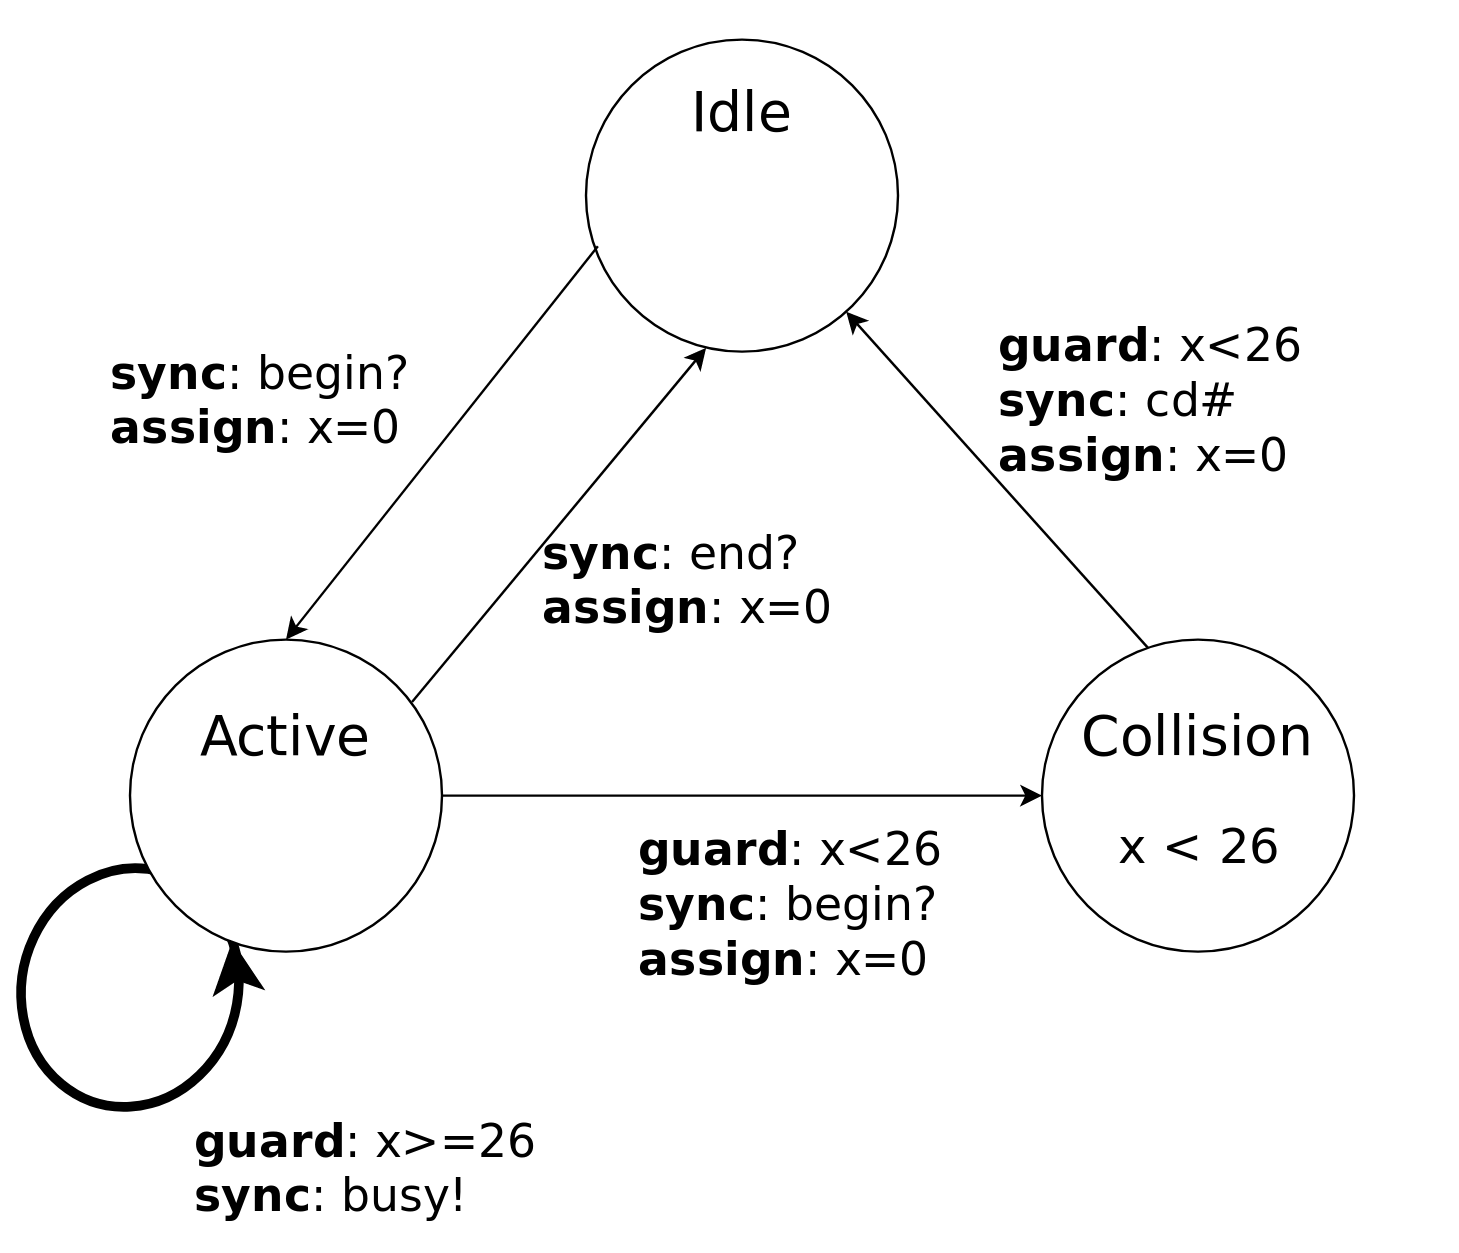
\includegraphics[width=0.6\textwidth]{csma-bus}
  \caption{CSMA Bus Automaton}
  \label{fig:csma-bus}
\end{figure}

Figure~\ref{fig:csma-bus} shows the TA diagrams used for the bus process. We have shown in
bold the new transition that was added to the standard version to improve the
quality of the benchmark. To simulate the ability of the sending processes to
detect when the bus is already in use, we have added a new transition to the bus
process that allows it to send a \textbf{busy} signal to another process when it
is in the active state and at least 26 time units have passed since the
beginning of the current transmission (26 is used to represent the delay for the
signal to propagate to other processes).

\begin{figure}[h]
  \centering
  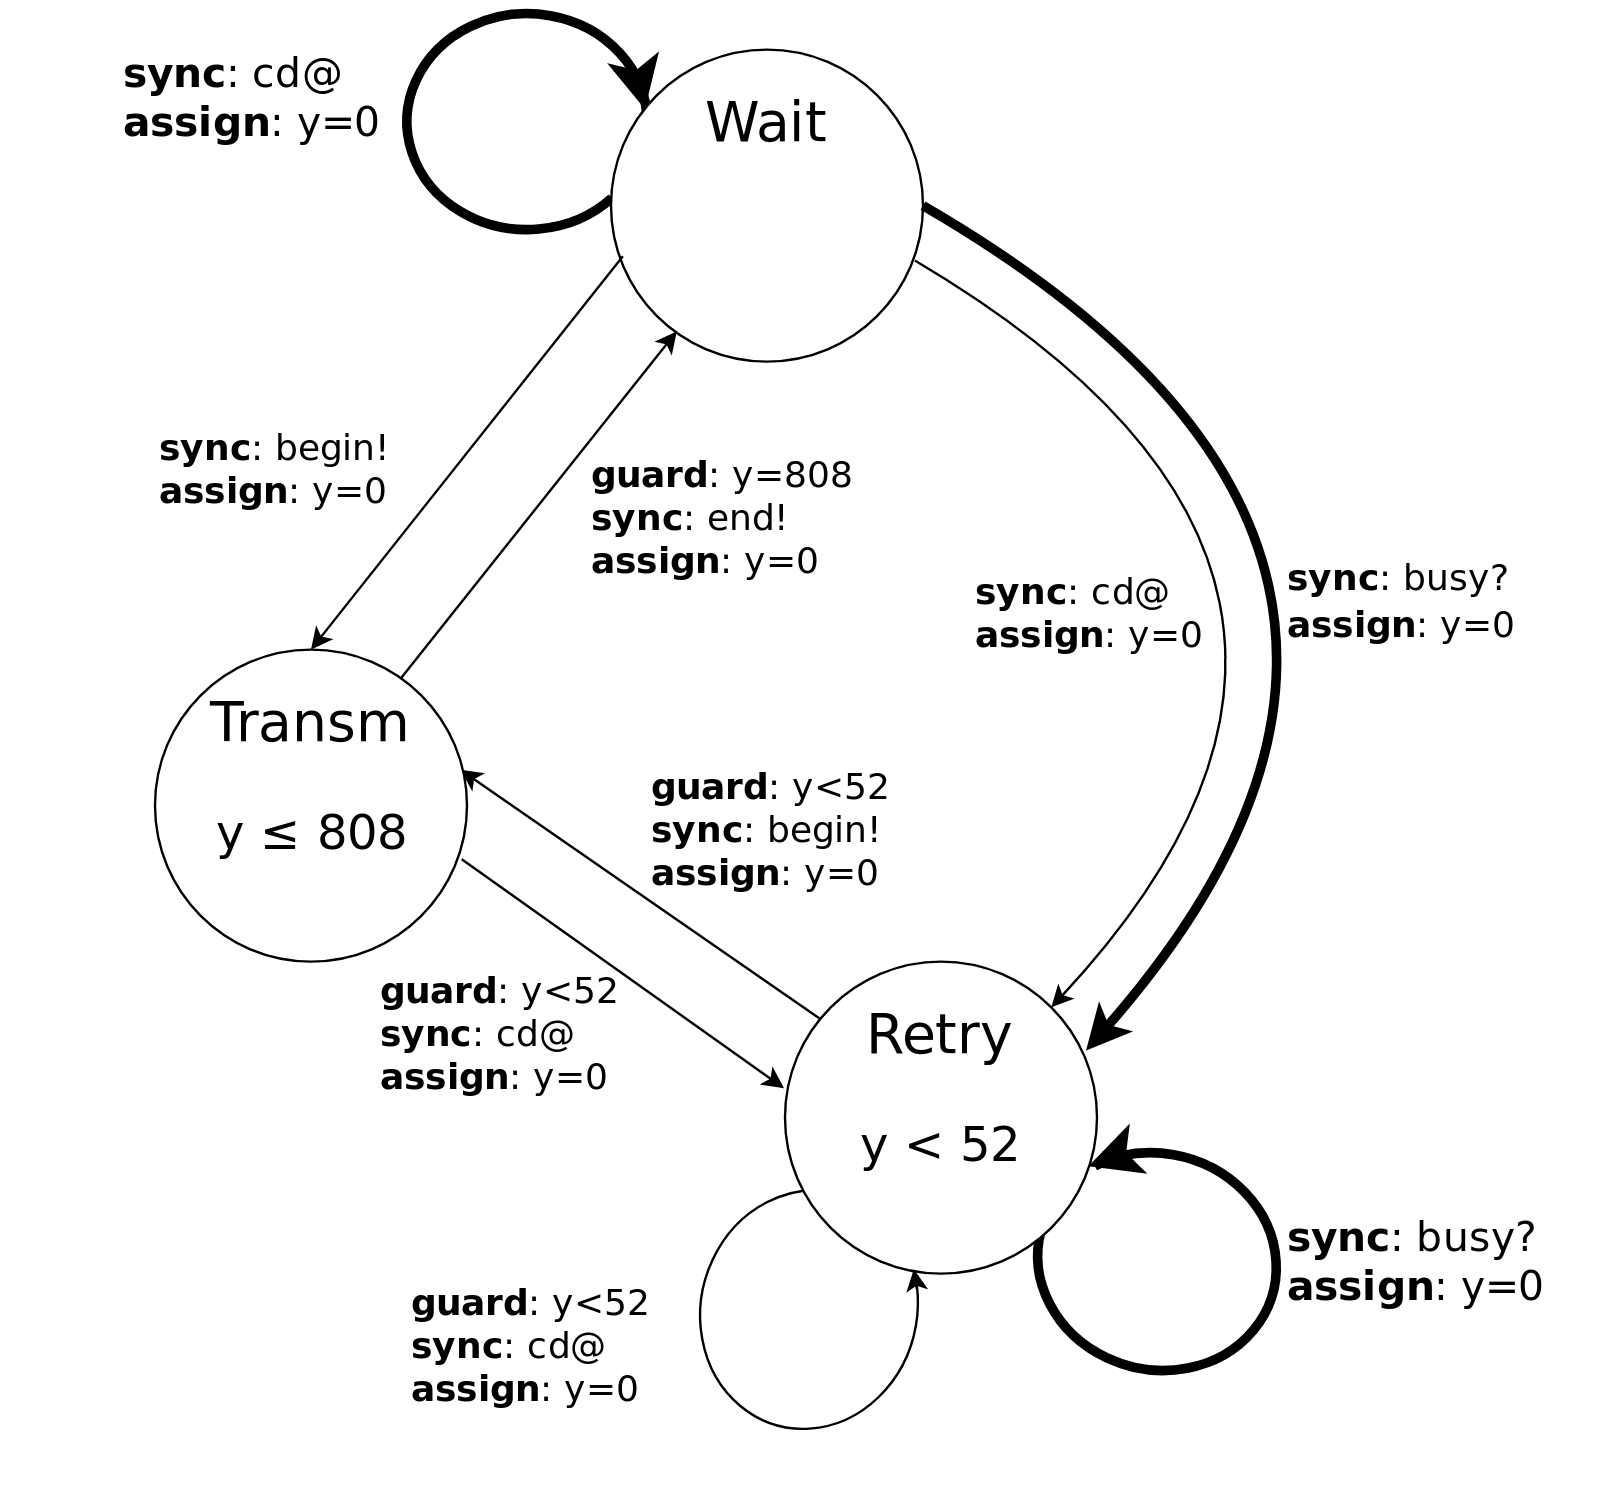
\includegraphics[width=0.7\textwidth]{csma-sender}
  \caption{CSMA Sender Automaton}
  \label{fig:csma-sender}
\end{figure}

Figure~\ref{fig:csma-sender} shows the diagram for the sending process. Again
the new additions are shown in bold. Note that each sending process has its own
unique clock, so that each process can reset its clock independently. In the
diagram for the sending processes we have added three new transitions. The first
keeps the TA in the waiting state, and synchronizes using the \textbf{cd} signal
(short for ``collision detected''). This allows the process to choose whether to
remain in the waiting state or move to the retry state when it receives this
broadcast synchronization signal. The other two new transitions concern the
added \textbf{begin} synchronization channel. The first allows a waiting process
that wishes to transmit to detect a transmission in-progress and transition
directly into the retry state. The final, and most crucial transition allows a
process in the retry state to detect that the bus is still busy, and reset its
clock. This allows it to remain in the retry state for the full 808 time units
needed for a complete transmission.

While running this experiment we discovered a previously unknown flaw in the
\aez\ encoding of the broadcast synchronization constraints. Therefore the
results are not directly comparable, as ta2smt must explore the entire search
space before returning a result of \textbf{sat}, while the \aez\ algorithm can
terminate after finding one (erroneous) counterexample. Rather than present
incomparable results, we have decided to instead present two runs of the ta2smt
encoding with different liveness and edge constraints.

\begin{table}[t]
\footnotesize
%\setstretch{0.6}
%\small
\center
\begin{tabular}{
r  r  r
r  r  r
r  r  r
r  r
}
\toprule
%\cline{3-11}
%\cline{3-11}
  \multicolumn{2}{c}{} &   \multicolumn{9}{c}{TACK ta2smt (Strong Transition
                         Liveness, Right-Closed Edges)}  \\
  \midrule
  \multicolumn{2}{c}{}  &    \multicolumn{9}{c}{$n$}  \\
  \midrule
\multicolumn{1}{c}{}  & k &    \multicolumn{1}{c}{\textbf{2}} & \multicolumn{1}{c}{\textbf{3}} & \multicolumn{1}{c}{\textbf{4}} & \multicolumn{1}{c}{\textbf{5}} & \multicolumn{1}{c}{\textbf{6}} & \multicolumn{1}{c}{\textbf{7}} & \multicolumn{1}{c}{\textbf{8}} & \multicolumn{1}{c}{\textbf{9}} & \multicolumn{1}{c}{\textbf{10}}  \\
%\cline{2-11}
%   \hline
\toprule
  \multirow{5}{*}{\rotatebox[origin=c]{90}{\textbf{live-csmacd}}}
     & \textbf{10} & 2.4 & 3.5 & 4.3 & 5.1 & 5.2 & 5.8 & 8.8 & 7.8 & 9.5 \\
     & \textbf{15} & 11.0 & 31.2 & 37.2 & 52.7 & 93.6 & 121.7 & 208.7 & 275.4 & 324.0 \\
     & \textbf{20} & 27.1 & 109.5 & 263.5 & 721.5 & 1778.3 & 2206.1 & 3616.7 & 5097.3 & 5068.9 \\
     & \textbf{25} &  \\
     & \textbf{30} &  \\
  \toprule
  \multicolumn{2}{c}{}  &   \multicolumn{9}{c}{TACK ta2smt (Unrestricted
                          Liveness, Open Edges)}  \\
    \midrule
  \multicolumn{2}{c}{}  &    \multicolumn{9}{c}{$n$}  \\
  \midrule
\multicolumn{1}{c}{}  & k &    \multicolumn{1}{c}{\textbf{2}} & \multicolumn{1}{c}{\textbf{3}} & \multicolumn{1}{c}{\textbf{4}} & \multicolumn{1}{c}{\textbf{5}} & \multicolumn{1}{c}{\textbf{6}} & \multicolumn{1}{c}{\textbf{7}} & \multicolumn{1}{c}{\textbf{8}} & \multicolumn{1}{c}{\textbf{9}} & \multicolumn{1}{c}{\textbf{10}}  \\
   \toprule
  \multirow{5}{*}{\rotatebox[origin=c]{90}{\textbf{live-csmacd}}}
     & \textbf{10} & 2.8 & 3.9 & 5.0 & 5.3 & 8.1 & 9.8 & 9.2 & 11.8 & 10.5 \\
     & \textbf{15} & 14.0 & 44.2 & 55.6 & 72.7 & 198.2 & 219.4 & 209.7 & 469.9 & 367.2 \\
     & \textbf{20} & 64.3 & 245.4 & 543.9 & 1188.7 & 2764.7 & 2037.6 & 4110.6 & $-$ & $-$ \\
     & \textbf{25} &  \\
     & \textbf{30} &  \\
%    \multicolumn{1}{|c|}{} &    U &  \multicolumn{2}{|c|}{} & \multicolumn{2}{|c|}{} & \multicolumn{2}{|c|}{} & \multicolumn{2}{|c|}{} & \multicolumn{2}{|c|}{} & \multicolumn{2}{|c|}{} & \multicolumn{2}{|c|}{} & \multicolumn{2}{|c|}{} & \multicolumn{2}{|c|}{}   \\
   \bottomrule
  \cline{1-11}
\end{tabular}
\caption[Time required to check the property of the CSMA/CD Protocol]{Time
  required to check the property of the CSMA/CD Protocol. A \cmark\ indicates
  the property is satisfied, a \xmark\ indicates that a counterexample was
  found. Blank entries indicate no result after two hours.}
\label{table:csmacd-results}
\end{table}

In Table~\ref{table:csmacd-results} we see the first run, which follows our
convention of using Strong Transition Liveness and Right-Closed edges. The
second run, however uses Unrestricted Liveness and Open edges. This means that
the second run has many more possibilities (valid traces) to consider, and we
would expect it to take a longer amount of time to verify the property. Once
again for small problem sizes the difference is minute, however although not as
drastic as the difference between \aez\ and ta2smt, there is still a significant
difference at higher bounds and higher numbers of agents.


\chapter{Conclusion}\label{conclusion}

We have presented a novel approach for encoding networks of Timed Automata
directly into BitVector logic, suitable for solving by state-of-the-art SMT
solvers. Building off of the work begun with the development of the TACK solver,
we retain TACK's approach of encoding MITL properties to be verified over the
network, while creating a more efficient model for the encoding of the network
itself. Rather than encode the TA network into \cltloc, we directly translate
the network terms and constraints into a combination of BitVector and
real-valued logic, written in the standard SMT-LIB2 language. One of the
original motivations for using \cltloc\ as an intermediate representation in
TACK was to create a common language that was both feasible to translate into
SMT form and expressive enough to easily support the encoding of additional
features. We have strived to make our encoding modular and easily accessible so
that future additions will not be hampered by the ``low-level'' nature of our
encoding.

In addition to re-implementing the translation of timed automata networks, we
have corrected several deficiencies in the original TACK implementation, and
the tool now supports the full variable constraint and variable assignment
grammars. In addition our implementation allows users to choose the desired
liveness and edge semantics at run-time. Furthermore our encoding eliminates the
unnecessary state BitVectors, creating a smaller search space for the SMT
solver. We are proud to present the implementation of this algorithm, which is
available for download at \url{https://github.com/fm-polimi/TACK} alongside the
original TACK encoding, as free software.

Empirical testing has revealed that our approach exhibits significant speedups
across several benchmarks when compared to the previous encoding. The results
seem to indicate that our approach is better suited to exploring models with
larger bounds, as the time necessary to solver larger and larger bounds grows
more slowly when compared with the \cltloc\ encoding.

\section{Future Work}

One potential future research direction is in similarly improving the encoding
of the MITL property files into BitVector logic. As seen in the TACK results,
the speedup achieved by our tool was weakest when the MITL property was the
largest, namely during the tests of Fischer liveness property six. Another
benefit to this re-implementation would be the potential inclusion of finite
traces (albeit with restrictions on the properties supported). This can already
be supported in the TA encoding by disabling the loop constraints, however
restrictions to the MITL encoding would be necessary to make this extension useful.

Another potential feature that could be more easily added is support for
automatically verifying that bounded integer variables are never assigned a
value outside of their bounds. Currently our BitVector implementation simply
allows variables to overflow, considering the burden of verifying the bounds to
fall on the user. However it would be relatively straightforward to increase the
size of the variable BitVectors so that an illegal assignment would no longer
overflow, and to then create a custom MITL property that asserts that the
variable never leaves its given bounds. Users could then check to see if their
bounds were in fact correct, and receive a trace showing the violation if one
existed.

\newpage

\bibliography{smtTranslation}
\bibliographystyle{ieeetr}

\end{document}
